
\def\spacingset#1{\renewcommand{\baselinestretch}%
	{#1}\small\normalsize} \spacingset{1}

\appendix
\setcounter{page}{1}
\begin{center}
{\bf \Large  Supplementary Material for\\``Estimating Heterogeneous Causal Effects of
  High-Dimensional Treatments:  Application to Conjoint Analysis''}

\vspace{0.5cm}
{ \large Max Goplerud \hspace{.5in} Kosuke Imai \hspace{.5in} Nicole E. Pashley}
\end{center}

\setcounter{equation}{0}
\setcounter{figure}{0}
\setcounter{theorem}{0}
\setcounter{lemma}{0}
\setcounter{section}{0}
\setcounter{table}{0}
\renewcommand {\theequation} {A\arabic{equation}}
\renewcommand {\thefigure} {A\arabic{figure}}
\renewcommand {\thealgorithm} {A\arabic{algorithm}}
\renewcommand {\thetable} {A\arabic{table}}
\medskip 

\section{The Details of the Immigration Conjoint Experiment}
\label{app:conjoint}

 \begin{table}[ht!]
    \centering\small
    \begin{tabular}{|p{0.25\linewidth}|p{0.12\linewidth}| p{0.58\linewidth}|}
    \hline
    Attribute &\# of Levels & Levels\\
     \hline
    Education & 7 & No formal education; Equivalent to completing fourth grade in the U.S.; Equivalent to completing eighth grade in the U.S.; Equivalent to completing high school in the U.S.; Equivalent to completing two years at college in the U.S.; Equivalent to completing a college degree in the U.S.; Equivalent to completing a graduate degree in the U.S.\\
    Gender & 2 & Female; Male\\
    Country of origin & 10 & Germany; France; Mexico; Philippines; Poland; India; China; Sudan; Somalia; Iraq\\
    Language & 4 & During admission interview, this applicant spoke fluent English; During admission interview, this applicant spoke broken English; During admission interview, this applicant tried to speak English but was unable; During admission interview, this applicant spoke through an interpreter\\
    Reason for Application & 3 &  Reunite with family members already in U.S.; Seek better job in U.S.; Escape political/religious persecution\\
    Profession & 11 & Gardener; Waiter; Nurse; Teacher; Child care provider; Janitor; Construction worker; Financial analyst; Research scientist; Doctor; Computer programmer\\
    Job experience & 4 & No job training or prior experience; One to two years; Three to five years\\
    Employment Plans & 4 & Has a contract with a U.S. employer; Does not have a contract with a U.S. employer, but has done job interviews; Will look for work after arriving in the U.S.; Has no plans to look for work at this time\\
    Prior Trips to the U.S. & 5 & Never been to the U.S.; Entered the U.S. once before on a tourist visa; Entered the U.S. once before without legal authorization; Has visited the U.S. many times before on tourist visas; Spent six months with family members in the U.S.\\
    \hline
    \end{tabular}\caption{Table 1 in \cite{hainmueller2015hidden}. All attributes for immigrants and their levels.}\label{tab:attributes}
\end{table}

\section{Propriety of the Structured Sparse Prior}
\label{sec:app_ssparse_prior}

The proof of propriety for the structured sparse prior used in our
paper is an application of Theorem~1 established in
\cite{goplerud2021sparsity} and is reproduced here.
\begin{theorem}[\cite{goplerud2021sparsity}] 
	\label{result:goplerud_1}
        Consider the following structured sparse prior on
        $\bm{\beta} \in \mathbb{R}^p$ with regularization strength
        $\lambda > 0$ penalizes $K$ linear constraints $\bm{d}_k$ and
        $L$ quadratic constraints $\bm{F}_\ell$ on the parameters
        where $\bm{F}_\ell$ is symmetric and positive
        semi-definite. The kernel of the prior is shown below.
  $$p(\bm{\beta}) \propto \exp\left(-\lambda \left[\sum_{k=1}^K
      |\bm{d}_k^\top \bm{\beta}| + \sum_{\ell=1}^L \sqrt{
        \bm{\beta}^\top \bm{F}_{\ell} \bm{\beta}}\right] \right)$$ Further
  define $\bm{D}^\top = [d_1, \cdots, d_K]^\top$ and
  $\bar{\bm{D}}^\top = [\bm{D}^\top, \bm{F}_1, \cdots, \bm{F}_L]$.
  Then, for $\lambda >0 $, the prior above is proper if and only if
  $\bar{\bm{D}}$ is full column rank.
\end{theorem}
In our specific case, we note that $K = 0$, $L = G$, and
$\lambda = \lambda \bar{\pi}_k^\gamma$. Prior propriety of
$p(\bm{\beta}_k \mid \{\bm{\phi}_k\}_{k=2}^K, \lambda)$, therefore,
can be determined by empirically investigating whether $\bar{\bm{D}}$,
i.e. the vertically stacked $\bm{F}_\ell$, is full column rank.

It is also possible to analytically show the propriety of the prior
distribution in all cases considered in this paper. We focus on the
case of $K = 1$ and arbitrary $\lambda > 0$ as the result follows
automatically for the case in our paper. 
\begin{result}
	\label{thm:proper_prior}
	Assume a structured sparse prior for a factorial or conjoint
        design with $J$ factors each with $L_j$ levels where all
        pairwise interactions are included and levels of each factor
        are encouraged to be fused together (i.e. the model in the
        main text). The kernel of the prior is shown below where
        $\bm{F}_g$ are as defined in the main text. 	
	$$k(\bm{\beta}) = \exp\left(-\lambda \sum_{g=1}^G \sqrt{\bm{\beta}^\top \bm{F}_g \bm{\beta}}\right)$$
	Assume that the linear sum-to-zero constraints
        $\bm{C}^\top \bm{\beta} = \bm{0}$ hold.  Then, the structured
        sparse prior on the unconstrained $\tilde{\bm{\beta}}$ such
        that $\tilde{\bm{\beta}} \in \mathcal{N}(\bm{C}^\top)$ is
        proper. Or, equivalently, the following result holds.
	$$\int_{\bm{\beta}: \bm{C}^\top \bm{\beta} = \bm{0}} k(\bm{\beta}) d\bm{\beta} < \infty.$$
\end{result}
\begin{proof}
  Let $\mathcal{B}_{\bm{C}^\top}$ represent a basis for the
  linear constraints $\bm{C}^\top$. The integral for evaluating
  propriety can be written as,
  \begin{equation*}
\int_{\tilde{\bm{\beta}}} \tilde{k}(\tilde{\bm{\beta}})
d\tilde{\bm{\beta}}\quad \text{where} \quad \tilde{k}(\tilde{\bm{\beta}}) =
\exp\left(-\lambda \sum_{g=1}^G
  \sqrt{\tilde{\bm{\beta}}^\top\mathcal{B}_{\bm{C}^\top}^\top \bm{F}_g
    \mathcal{B}_{\bm{C}^\top} \tilde{\bm{\beta}}}\right). 
\end{equation*}
Note that $\bm{F}_g$ can be expressed as a sum of $N_g$ outer products
of $|\bm{\beta}|$-length vectors of the form
$\bm{l}_i \in \{-1, 0, 1\}$ where $-1$ and $1$ correspond to the two
terms that are fused together and all other elements are $0$, i.e.,
$ \bm{F}_g = \sum_{g'=1}^{N_g} \bm{l}_{g'}\bm{l}_{g'}^\top$. Thus, one
can define a matrix
$\bm{Q}_g^\top = \left[\bm{l}_1, \cdots, \bm{l}_{N_g}\right]$ such
that $\bm{Q}_g^\top \bm{Q}_g = \bm{F}_g$, which allows us to rewrite
% where each row of $\bm{Q}_g$ has exactly one element as `1' and one as `-1' and the rest are zero. $\bm{Q}_g$ is an orientated incidence matrix of a graph $\mathcal{G}_g$ where each node is a coefficient in $\bm{\beta}$. 
$\tilde{k}(\tilde{\bm{\beta}})$ as:
$$\tilde{k}(\tilde{\bm{\beta}}) = \exp\left(-\lambda \sum_{g=1}^G
  \sqrt{\tilde{\bm{\beta}}^\top
    \left[\mathcal{B}_{\bm{C}^\top}\right]^\top \bm{Q}_g^\top \bm{Q}_g
    \mathcal{B}_{\bm{C}^\top} \tilde{\bm{\beta}}}\right).$$

By applying Theorem~\ref{result:goplerud_1} and noting that the
nullspaces of $\bm{A}^T\bm{A}$ and $\bm{A}$ are identical, the
integral of $\tilde{k}(\tilde{\bm{\beta}})$ is finite if and only if
$\bm{Q}\mathcal{B}_{\bm{C}^\top}$ is full column rank, where
$\bm{Q}^\top = [\bm{Q}^\top_1, \cdots, \bm{Q}^\top_G]$.  We
demonstrate this fact in two steps.  First, there exists a permutation
matrix $\bm{P}_{Q}$ such that $\bm{P}_Q \bm{Q} $ has a block diagonal
structure with $J+1$ diagonal blocks. The first $J$ blocks
corresponding to the main terms for each factor $j$ and the last block
corresponds to all interaction terms. The nullspace of each block is
spanned by the vector $\bm{1}$ as the corresponding block of
$\bm{P}_Q\bm{Q}$ is a (transposed) orientated incidence matrix of a
fully connected graph. Thus, the nullspace of $\bm{P}_Q \bm{Q}$, and
hence $\bm{Q}$, is spanned by the $J+1$ columns of a block diagonal
matrix with $\bm{1}$ on each block.  Second, consider the linear
constraints $\bm{C}^\top \bm{\beta} = \bm{0}$.  The only vector to
satisfy this constraint and lie in the nullspace of $\bm{Q}$ must be
$\bm{0}$ as, for each block, the only vector proportional to $\bm{1}$
and satisfying the corresponding sum-to-zero constraints must be
$\bm{0}$. Thus, $\bm{Q}\mathcal{B}_{\bm{C}^\top}$ is full column rank
and the prior is proper.
\end{proof}

\section{Derivations for the Basic Model}
\label{sec:app_derivations}

This section derives a number of results for the basic model. It first
restates the main results concerning the elimination of the linear
constraints $\bC^\top \bm{\beta}_k = \bm{0}$. Then, it derives the
Expectation Maximization algorithm, our measure of degrees of freedom,
and some additional computational improvements used to accelerate
estimation.  In the following, with a slight abuse of notation, we use
$\bm{t}_i$ to denote the corresponding vector of indicators for
whether certain treatments or interactions are present (i.e. stacking
all $I(T_{ij} = 1)$, etc. from Equation~\ref{eq:define_lp}).  In
addition, we use $\psi_{ik}$ to indicate the linear predictor for
observation $i$ and cluster $k$.

\subsection{Removing the Linear Constraints}
\label{sec:app_derivation_LC}

The inference problem in the main text is presented as an optimization
problem subject to linear constraints on the coefficients
$\bm{\beta}_k$. We note that inference is noticeably easier if these
are eliminated via a transformation of the problem to a
lower-dimensional one by noting that $\bm{\beta}_k$ must lie in the
null space of the constraint matrix $\bm{C}^\top$. Define
$\tilde{\bm{\beta}}_k = \left(\mathcal{B}_{\bC^\top}^\top
  \mathcal{B}_{\bC^\top}\right)^{-1}
\mathcal{B}_{\bC^\top}^\top\bbeta_k$ where $\mathcal{B}_{\bC^\top}$ is
a basis for the null space of $\bC^\top$. Given this, the problem can
be solved in terms of the unconstrained
$\tilde{\bm{\beta}}_k \in \mathbb{R}^{p-\mathrm{rank}(\bC^\top)}$. The
treatment design vectors
($\tilde{\bm{t}}_i = \mathcal{B}_{\bC^\top} \bm{t}_i$) and penalty
matrices ($\tilde{\bF}_g$ as
$\mathcal{B}_{\bC^\top}^\top \bF_g \mathcal{B}_{\bC^\top}$) are
adjusted and then the augmented problem can be written in
Equations~\eqref{eq:augmented1}~and~\eqref{eq:augmented2}. The new
linear predictor is
$\psi_{i,k} = \left[\tilde{\bm{t}}_i\right]^\top
\tilde{\bm{\beta}}_{Z_i} + \mu$.

Note that the only difference between the unconstrained and
constrained problem is the choice of treatment design matrix. Given
this similarity and to reduce the burden of notation, we thus present
all results herein dropping the ``tilde'' notation and note that, once
estimated, $\tilde{\bm{\beta}}_k$ is projected back into the original
space for the reported coefficients, average marginal component effects,
etc. Given Appendix~\ref{sec:app_uncertainty}'s results on
approximating $\tilde{\bm{\beta}}_k$ as normal, $\bm{\beta}_k$ will
have a (singular) normal distribution distribution.

\subsection{Expectation Maximization Algorithm}
\label{sec:app_derivation_EM}

Assume that we have the model after the linear constraints have been removed as discussed above. We begin with the cycle of the AECM algorithm for updating $\{\bm{\beta}_k\}_{k=1}^K$ given $\{\bm{\phi}_{k=2}^K\}$.  The model with triple augmentation is shown below, mirroring Equation~\eqref{eq:aecm_ebeta} from the main text.
\begin{subequations}
	\label{app_eq:augmented}
	\begin{alignat}{2}
	&p(Y_i, \omega_{i} \mid Z_i) = \frac{1}{2} \exp\left[\left(Y_i - \frac{1}{2}\right)
          \psi_{i, Z_i} - \frac{\omega_{i}}{2} \psi_{i, Z_i}^2\right]
        f_{PG}(\omega_{i} \mid 1, 0) \\ 
	&p(\bm{\beta}_k, \{\tau^2_{gk}\} \mid \lambda, \{\bm{\phi}_k\}) \propto \exp\left[-\frac{1}{2}{\bm{\beta}}_k^\top\left(\sum_{g=1}^K \frac{{\bm{F}}_{g}}{\tau^2_{gk}}\right) {\bm{\beta}}_k\right] \cdot \prod_{g=1}^G \frac{\exp\left(-\left[\lambda \bar{\pi}_k\right]^2/2 \cdot \tau^2_{gk}\right)}{\sqrt{\tau^2_{gk}}} \\
	&Z_i \sim \mathrm{Multinomial}\left(1, \bm{\pi}_i\right); \quad \psi_{ik} = \bm{t}_i^\top \bm{\beta}_k + \mu
	\end{alignat}
\end{subequations}

We treat $\{\omega_i, Z_i\}_{i=1}^N$ and $\{\tau^2_{gk}\}$ as missing
data to be used in the $E$-Step and $\bm{\beta}_k$ as parameters to be
optimized in an $M$-Step. For this cycle of the AECM algorithm, we hold $\bm{\phi}$ constant. The $E$-Step can be computed by noting that $p(\omega_i, Z_i \mid Y_i, \bm{\theta})$ and $p(\tau^2_{gk} \mid \bm{\theta})$ are conditionally independent across $i$ and $gk$. The distributions are shown below,
\begin{subequations}
\begin{align}
p(\tau^{-2}_{gk} \mid \bm{\theta}) &\sim \mathrm{InverseGaussian}\left(\frac{\lambda}{\sqrt{\bm{\beta}_k^\top\bm{F}_g\bm{\beta}_k}}, \quad \lambda^2\right), \\
p(Z_i = k \mid Y_i, \bm{\theta}) &\propto p_{ik}^{Y_i} (1-p_{ik})^{1-Y_i} \pi_{ik}; \quad p_{ik} = \frac{\exp(\psi_{ik})}{1+\exp(\psi_{ik})}, \\
p(\omega_i \mid Z_i = k, \bm{\theta}) &\sim \mathrm{PG}\left(1, \psi_{ik}\right).
\end{align}
\end{subequations}
The relevant expectations are shown below,
\begin{subequations}
\begin{align}
& \E\left(\tau^{-2}_{gk}\right) = \frac{\lambda}{\sqrt{\bm{\beta}_k^\top\bm{F}_g\bm{\beta}_k}}; \\
& \E (z_{ik}) = \E\left[I(Z_i = k)\right] = \frac{p_{ik}^{Y_i} (1-p_{ik})^{1-Y_i} \pi_{ik}}{\sum_{\ell=1}^K p_{i\ell}^{Y_i} (1-p_{i\ell})^{1-Y_i} \pi_{i\ell}} \\
& \E (\omega_{i} \mid Z_i = k) = \frac{1}{2\psi_{ik}} \tanh\left(\frac{\psi_{ik}}{2}\right)
\end{align}
\end{subequations}

Note that as $\bm{\beta}_k^\top \bm{F}_g \bm{\beta}_k$ approaches
zero, $\E(\tau^{-2}_{gk})$ approaches infinity. To prevent numerical
instability, we rely on the strategy in \cite{goplerud2021sparsity}
(inspired by \citealt{polson2011svm}) where once it is sufficiently
small, e.g. below $10^{-4}$, and thus the restriction is almost
binding, we ensure that restriction holds in all future iterations. We
do so by adding a quadratic constraint
$\bm{\beta}_k^\top \bm{F}_g \bm{\beta}_k = 0$. Note that this again
implies that $\bm{\beta}_k$ lies in the nullspace of $\bm{F}_g$ and
thus with an additional transformation, it can be removed and the
problem be solved in an unconstrained space with a modified design.

With these results, the $Q_\beta$-function can be thus expressed as the
expectation of the logarithm of the augmented posterior where we suppress all terms
that do not depend on $\bm{\beta}_k$ and all expectations depend on prior value $\bm{\theta}^{(t)}$. Recall that $\bm{\beta} = \{\{\bm{\beta}_k\}_{k=1}^K, \mu\}$.

\begin{align}
  & Q_\beta\left(\bm{\beta}, \bm{\theta}^{(t)}\right)\nonumber  \\
  = &\sum_{i=1}^N \left[\sum_{k=1}^K \E(z_{ik})\left\{\left(Y_i -
      \frac{1}{2}\right) \psi_{ik} - \E(\omega_i \mid Z_i = k)
      \frac{\psi^2_{ik}}{2}\right\} \right]  + \sum_{k=1}^K -\frac{1}{2}
      \bm{\beta}_k^\top \left[\sum_{g=1}^K \bm{F}_g \cdot
     \E(1/\tau^2_{gk})\right] \bm{\beta}_k + \text{const.} \label{eq:q_func}
\end{align}

From the above, define a vector that concatenates
$\check{\bm{\beta}}^\top = [\mu, \bm{\beta}_1, \cdots,
\bm{\beta}_K]^\top$. We can create a corresponding design
$\check{\bm{T}} = [\bm{1}_{N}, \bm{I}_K \otimes \bm{T}]$
where $\bm{T}^\top = [\bm{t}_1, \cdots, \bm{t}_N]$. We further create
a corresponding diagonal weight matrix
$\check{\bm{\Omega}} =
\mathrm{diag}\left(\{\{\E(z_{ik})\E(\omega_{i}\mid Z_i =
  k)\}_{i=1}^N\}_{k=1}^K\right)$. Further, we can create the combined
ridge penalty
$\bm{\mathcal{R}} = \mathrm{blockdiag}\left(\{0,
  \{\bm{R}_k\}_{k=1}^K\}\right)$ where
$\bm{R}_k = \sum_g \bm{F}_g \E(\tau^{-2}_{gk})$. Finally, we can
create the augmented outcome
$\check{\bm{Y}} = \{\{\E(z_{ik}) (Y_i - 1/2)\}_{i=1}^N\}_{k=1}^K$. With
this in hand, we can rewrite the $Q_\beta$ function as proportional to
the following ridge regression problem and the corresponding update in
the $M$-Step.
\begin{align*}
  Q_\beta\left(\bm{\beta};
  \bm{\theta}^{(t)}\right) & = \check{\bm{Y}}^\top
                               \left(\check{\bm{T}}
                               \check{\bm{\beta}}\right) - \frac{1}{2}
                               \check{\bm{\beta}}^\top
                               \check{\bm{T}}^\top \check{\bm{\Omega}}
                               \check{\bm{T}} \check{\bm{\beta}} -
                               \frac{1}{2} \check{\bm{\beta}}^\top
                               \bm{\mathcal{R}} \check{\bm{\beta}}  + \text{const.},\\
  \check{\bm{\beta}}^{(t+1)} &= \left(\check{\bm{T}}^\top \check{\bm{\Omega}} \check{\bm{T}} + \bm{\mathcal{R}}\right)^{-1} \check{\bm{T}}^\top \check{\bm{Y}}.
\end{align*}
Note that since $\check{\bm{\Omega}}$, $\check{\bm{Y}}$, and
$\mathcal{\mathbb{R}}$ depend on $\bm{\theta}^{(t)}$, we can think
about this algorithm as follows where we denote their dependence on
prior values with the superscript $(t)$.
$$\check{\bm{\beta}}^{(t+1)}  = \left(\check{\bm{T}}^\top \check{\bm{\Omega}}^{(t)} \check{\bm{T}} + \bm{\mathcal{R}}^{(t)}\right)^{-1} \check{\bm{T}}^\top \check{\bm{Y}}^{(t)} $$

In practice, we rely on a generalized EM algorithm where $Q_\beta$ is
improved versus maximized for computational reasons; we do so using a
conjugate gradient solver initialized at
$\check{\bm{\beta}}^{(t)}$. The update for $\{\bm{\phi}_k\}_{k=2}^K$
is shown in the main text; as is required for AECM algorithms, it requires a re-computation of the $E$-Step for $\E(z_{ik})$ that depends on $\bm{\beta}^{(t+1)}$. We use L-BFGS-B for a few steps to improve the objective.

\subsection{Degrees of Freedom}
\label{sec:app_derivations_df}

We note that our procedure for estimating $\check{\bm{\beta}}^{(t)}$
appears similar to the results in \cite{oelker2017uniform} where
complex regularization and non-linear models can be recast as a
(weighted) ridge regression. Using that logic, we take the trace of
the ``hat matrix'' implied by our algorithm at stationarity to
estimate our degrees of freedom. We also adjust upwards the degrees of
freedom by the number of moderator coefficients (e.g.,
\citealt{khalili2010mixture,chamroukhi2019regularized}).

Equation~\eqref{eq:df} shows our procedure where $\bm{\mathcal{R}}$
and $\check{\bm{\Omega}}$ contain expectations calculated at
convergence. $p_x$ denotes the number of moderators, i.e. the
dimensionality of $\bm{\phi}_k$. Before evaluating
Equation~\eqref{eq:df}, for any two factor levels that are
sufficiently close (e.g.,
$\sqrt{\bbeta_k^\top\bF_g \bbeta_k} < 10^{-4}$), we assume they are
fused together and consider it as an additional linear constraint on
the parameter vector $\bm{\beta}_k$.

\begin{equation}
\label{eq:df}
\begin{split}
&\mathrm{df} = \mathrm{tr}\left[\left(\check{\bm{T}}^\top \check{\bm{\Omega}} \check{\bm{T}} + \bm{\mathcal{R}}\right)^{-1} \check{\bm{T}}^\top \check{\bm{\Omega}} \check{\bm{T}}\right] + p_x \left(K - 1\right)
\end{split}
\end{equation}

From this, we can calculate a BIC criterion. We seek to find the
regularization parameter $\lambda$ that minimizes this criterion. To
avoid the problems of a naive grid-search, we use Bayesian model-based
optimization that attempts to minimize the number of function
evaluations while searching for the value of $\lambda$ that minimizes
the BIC (\texttt{mlrMBO}; \citealt{bischl2018mlrmbo}). We find that
with around fifteen model evaluations, the optimizer can usually find
a near optimal value of $\lambda$.

\subsection{Computational Improvements}
\label{sec:app_derivations_improve}

While the algorithm above provides a valid way to locate a posterior
mode, our estimation problem is complex and
high-dimensional. Furthermore, given the complex posterior implied by
mixture of experts models, we derived a number of computational
strategies to improve convergence. We use the SQUAREM algorithm
(\citealt{varadhan2008simple}) and a generalized EM algorithm to
update $\bm{\beta}$ using a conjugate gradient approach and
$\bm{\phi}$ using a few steps of L-BFGS-B.

We also outline a way to deterministically initialize the model to provide stability and, again, speed up estimation on large problems. To do this, we adapt the procedure from \cite{murphy2020init} for initializing mixture of experts: (i) initialize the clusters using some (deterministic) procedure (e.g. spectral clustering on the moderators); (ii) using only the main effects, estimate an EM algorithm---possibly with hard assignment at the $E$-Step (CEM; \citealt{celeux1992classification}); (iii) iterate until the memberships have stabilized. Use those memberships to initialize the model. This has the benefit of having a deterministic initialization procedure where the cluster members are based on the moderators but guided by which grouping seem to have sensible treatment effects, at least for the main effects. Given the memberships, update $\bm{\beta}$ using a ridge regression and $\bm{\phi}$ using a ridge regression and take those values as $\bm{\beta}^{(0)}$ and $\bm{\phi}^{(0)}$.



\section{Extensions to the Basic Model}
\label{sec:app_extensions}

As noted in the main text, there are five major extensions to the basic model that applied users might wish to include:

\begin{enumerate}
	\item Repeated tasks (observations) for a single individual
	\item A forced-choice conjoint experiment
	\item Survey  to weight the sample estimate to the broader population
	\item Adaptive weights for each penalty
	\item Latent overlapping groups
\end{enumerate}

All can be easily incorporated into the proposed framework above. This
section outlines the changes to the underlying model.

\subsection{Repeated Observations}
\label{sec:app_extensions_repeat}

This modification notes that in factorial and conjoint experiments it
is common for individuals to perform multiple tasks. Typically, the
number of tasks $N_i$ is similar across individuals. The updated
likelihood for a single observation $i$ is shown below; we show both
the observed and complete case. $y_{it}$ represents the choice of
person $i$ on task $t \in \{1, \cdots, N_i\}$; $p_{itk}$ is the
probability of $Y_{it} = 1$ if person $i$ was in cluster $k$. 
\begin{align}
  &L\left(\{Y_{it}\}_{t=1}^{N_i}\right) = \sum_{k=1}^K \pi_{ik} \left[\prod_{t=1}^{N_i} p_{itk}^{Y_{it}} (1-p_{itk})^{1-Y_{it}} \right]; \quad p_{itk} = \frac{\exp(\psi_{itk})}{1+\exp(\psi_{itk})}; \quad \psi_{itk} = \bm{t}_{it}^\top\bm{\beta}_k + \mu 
\label{app_eq:repeated} \\
  &L^c(\{y_{it}, \omega_{it}\} \mid Z_i) = \prod_{t=1}^{N_i}
    \left[\frac{1}{2} \exp\left\{\left(Y_{it} - \frac{1}{2}\right)
    \psi_{i, Z_i} - \omega_{it} \frac{\psi_{it,Z_i}^2}{2}\right\}
    f_{PG}(\omega_{it} \mid 1, 0) \right]  
\end{align}

Note that because of the conditional independence of
$(y_{it}, \omega_{it})$ given $Z_i$ and the parameters, the major
modifications to the EM algorithm is that the $E$-Step must account
for all $t$ observations, i.e. the terms summed in
Equation~\eqref{app_eq:repeated}. Some additional book-keeping is
required in the code as the design of the treatments has
$\sum_{i=1}^N N_i$ rows whereas the design of the moderators has $N$
rows. Repeated observations can be easily integrated into the
uncertainty estimation procedure outlined below.

\subsection{Forced Choice Conjoint Design}
\label{sec:app_extensions_forced}

A popular design of a conjoint experiment is the forced choice design
where the respondents are required to choose between two profiles.
Therefore, the researcher does not observe an outcome for each profile
separately, but rather a single outcome is observed for each pair
indicating which is preferred. \cite{egam:imai:19} show that this can
be easily fit into the above framework with some adjustment.
Specifically, the model is modified to difference the indicators of
the treatment levels for the pair of profiles (subtracting, e.g., the
levels of the profile presented on the left from those of the profile
presented on the right). The intercept for this model can be
interpreted as a preference for picking a profile presented in a
particular location.  With this modification, estimation proceeds as
before.

\subsection{Standardization Weights}
\label{sec:app_extensions_standardization}

An additional modification to the problem is to weight the
penalty. This could be done for two reasons.  First, there is an issue
of the columns having different variances/Euclidean norms because of
the different number of factor levels $L_j$. Second, it is popular to
weight the penalty based on some consistent estimator (e.g. ridge
regression) to improve performance and, in simpler models, can be
shown to imply various oracle properties
(e.g. \citealt{zou2006adaptive}). We leave the latter to future
exploration.

Define $\xi_{gk}$ as a positive weight for the $g$-th penalty and the
$k$-th cluster. The kernel of the penalty is modified to include
them. 
\begin{equation}
\ln p(\bm{\beta}_k \mid \lambda, \gamma, \{\bm{\phi}_k\}) \propto -\lambda \bar{\pi}_k^\gamma \sum_{g=1}^G \xi_{gk} \sqrt{\bm{\beta}_k^\top \bm{F}_g \bm{\beta}_k}
\end{equation}
This has no implication on the rank of the stacked $\bm{F}_g$ (and
thus the results in Appendix~\ref{sec:app_ssparse_prior}) as they are
all positive and thus only slightly modify the $E$-Step. 

We employ weights in all of our analyses to account for the fact that
different factors $j$ may have different number of levels $L_j$. We
use a generalization of the weights in \cite{bondell2009anova} to the
case of penalized \emph{differences}. Specifically, consider the
over-parameterized model in Appendix~\ref{sec:app_log} where the
penalty can be written entirely on the differences
$\bm{\delta}_{\mathrm{Main}}$, $\bm{\delta}_{\mathrm{Int}}$,
$\bm{\delta}_{\mathrm{Main-Copy}}$.  Note that each of those penalties
has a simple (group) LASSO form and thus we adopt the approach in
\cite{lim2015learning} of weighting by the Frobenius norm of the
associated columns in $\bm{T}_{\mathrm{LOG}}$, i.e. the
over-parameterized design matrix. At slight abuse of notation, define
$[\bm{T}_{\mathrm{LOG}}]_g$ as the columns of $\bm{T}_{\mathrm{LOG}}$
corresponding to the differences penalized in the (group) lasso $g$,
the weight can be expressed as follows:
$$\xi_{gk} = \frac{1}{\sqrt{N}}||~\left[\bm{T}_{\mathrm{LOG}}\right]_{g} ||_F$$
Ignoring the factor of $\sqrt{N}$, this exactly recovers the weight proposed in \cite{bondell2009anova} in the non-latent-overlapping non-interactive model of $(L_j + 1)^{-1} \sqrt{N^j_{l} + N^j_{l'}}$ where $N^j_l$, $N^j_{l'}$ are the number of observations for factor $j$ in level $l$ and level $l'$ that are being encouraged to fuse together by the penalty in group $g$.



\subsection{Latent Overlapping Groups}
\label{sec:app_log}

One feature of the above approach is that our groups are highly
overlapping. \cite{yan2017hierarchical} suggest that, in this setting,
a different formulation of the problem may result in superior
performance (see also \citealt{lim2015learning}). Existing work on the
topic has focused on group LASSO penalties (e.g. $\bm{F}_g = \bm{I}$)
and thus some modifications are needed for our purposes. To address
this, we note that we can again recast our model in an equivalent
fashion.  Instead of penalizing
$\sqrt{\bm{\beta}_k^\top\bm{F}_g \bm{\beta}_k}$, we can penalize the
vector of differences between levels as long as we also impose linear
constraints to ensure that the original model is maintained.

Consider a simple example with two factors each with two levels
$\{1,2\}$ and $\{A,B\}$.  The relevant differences are defined such
that $\delta^j_{1-2} = \beta^j_{1} - \beta^j_2$ and
$\delta^{jj'}_{(lm) - (l'm')} = \beta^j_{l,m} -
\beta^{j'}_{l',m'}$. The equivalent penalty can be imposed as follows:
\begin{equation}
\begin{split}
&\sqrt{\left(\delta^j_{1-2}\right)^2 + \left(\delta^{jj'}_{(1A) - (2A)}\right)^2 + \left(\delta^{jj'}_{(1B)-(2B)}\right)^2} = \sqrt{\bm{\delta}^\top \bm{\delta}}; \quad \bm{\delta} = \left(\begin{array}{c} \delta^j_{1-2} \\ \delta^{jj'}_{(1A)-(2A)} \\ \delta^{jj'}_{(1B)-(2B)} \end{array}\right) \\
&\mathrm{such~that}~\left[\begin{array}{l} \delta^j_{1-2} \\ \delta^{jj'}_{(1A)-(2A)} \\ \delta^{jj'}_{(1B)-(2B)} \end{array}\right] = \left[\begin{array}{lll} \beta^j_1 - \beta^j_2 \\ \beta^{jj'}_{1A} - \beta^{jj'}_{2A} \\ \beta^{jj'}_{1B} - \beta^{jj'}_{2B} \end{array}\right]
\end{split}
\end{equation} 
The latent overlapping group suggests a slight modification.  In
addition to the above penalization of the $\ell_2$ norm of the main
and interactive differences,\footnote{Note the related ``hierarchical
  group LASSO'' would add separate individual penalties for each of
  the interactions. It is easy to include that in our approach.} it
duplicates the main effect and penalizes it separately while ensuring
that all effects maintain the accounting identities between the
``latent'' groups and the overall effect. Specifically, it modifies
the above penalty to duplicate the column corresponding to
$\delta^j_{1-2}$ and adds a new parameter
$\delta^j_{(1-2)-\mathrm{Copy}}$.

\begin{equation}
\begin{split}
\sqrt{\bm{\delta}^\top\bm{\delta}} + |\delta^j_{(1-2)-\mathrm{Copy}}| \quad \mathrm{such~that}~\left[\begin{array}{l} \delta^j_{1-2} \\ \delta^{jj'}_{(1A)-(2A)} \\ \delta^{jj'}_{(1B)-(2B)} \end{array}\right] + \left[\begin{array}{l} \delta^j_{(1-2)-\mathrm{Copy}} \\ 0 \\ 0 \end{array}\right] = \left[\begin{array}{lll} \beta^j_1 - \beta^j_2 \\ \beta^{jj'}_{1A} - \beta^{jj'}_{2A} \\ \beta^{jj'}_{1B} - \beta^{jj'}_{2B} \end{array}\right]
\end{split}
\end{equation} 

Scoping out to the full problem, define $\bm{\delta}_{\mathrm{Main}}$
as the main effect differences, e.g. $\delta^j_{1-2}$, and
$\bm{\delta}_{\mathrm{Int}}$ as the interaction differences and
$\bm{D}_{\mathrm{Main}}$ as the matrix such that
$\bm{D}_{\mathrm{Main}} \bm{\beta} = \bm{\delta}_{\mathrm{Main}}$, and
$\bm{D}_{\mathrm{Int}}$ as the corresponding matrix to create the
vector of interactions. Define $\bm{\delta}_{\mathrm{Main}-g}$ as the
sub-vector of $\bm{\delta}_{\mathrm{Main}-g}$ that corresponds to the
(main) effect differences between levels $l$ and $l'$ of factor $j$
penalized by $\bm{F}_g$ in the original notation. Similarly define
$\bm{\delta}_{\mathrm{Int}-g}$ and
$\bm{\delta}_{\mathrm{Main-Copy}-g}$.

\begin{equation}
\begin{split} &p(\bm{\beta},\bm{\delta}_{\mathrm{Main}}, \bm{\delta}_{\mathrm{Int}}, \bm{\delta}_{\mathrm{Main-Copy}}) =  \sum_{g=1}^G \sqrt{\bm{\delta}_{\mathrm{Main}-g}^T \bm{\delta}_{\mathrm{Main}-g} +  \bm{\delta}_{\mathrm{Int}-g}^T \bm{\delta}_{\mathrm{Int}-g}} +\sum_{g'=1}^{G} \sqrt{\left[\bm{\delta}_{\mathrm{Main-Copy}-g}\right]^2}\\
  &\mathrm{s.t.} \quad \left[\begin{array}{llll} \bm{C}^\top & \bm{0} & \bm{0} & \bm{0} \\ \bm{D}_{\mathrm{Main}} & -\bm{I} & \bm{0} & -\bm{I} \\ \bm{D}_{\mathrm{Int}} & \bm{0} & -\bm{I} & \bm{0} \end{array}\right] \left[\begin{array}{l} \bm{\beta} \\ \bm{\delta}_{\mathrm{Main}} \\ \bm{\delta}_{\mathrm{Int}} \\ \bm{\delta}_{\mathrm{Main-Copy}} \end{array}\right] = \bm{0} \end{split}
\end{equation} 

This also requires a modification of the design matrix $\bm{T}$ to ensure that (i) its dimensionality conforms with the expanded parameter vector and (ii) that for any choice of the expanded parameter that satisfies the constraints, the linear predictor for all observation (and thus the likelihood) is unchanged. Consider first the simple case without latent-overlapping groups. In this case, following \cite{bondell2009anova}, note that the expanded design can be expressed as $\tilde{\bm{T}} = \bm{T}\tilde{\bm{M}}^\dagger$ where $\tilde{\bm{M}}^\top = [ \bm{I}, \bm{D}_{\mathrm{Main}}^\top, \bm{D}_{\mathrm{Int}}^\top]$ and $\tilde{\bm{M}}^\dagger$ is a left-inverse of $\tilde{\bm{M}}$. The latent-overlapping group formulation is a simple extension; we copy the columns of $\tilde{\bm{T}}$ that correspond to $\bm{\delta}_{\mathrm{Main}}$ and append them to get $\bm{T}_{\mathrm{LOG}}$.

With this new design and parameterization in hand, we can again use the above results on projecting out the linear constraints to turn the problem into inference on an unconstrained vector $\bm{\beta}_k$ with a set of positive semi-definite constraints $\{\bm{F}_g\}_{g=1}^{2G}$ and inference proceeds identically to before.


\section{Estimators}\label{append:amce_acie_der}

Here we provide further details on the estimators.  In particular, we
discuss estimation of Average Marginal Component Effects (AMCEs) and
Average Marginal Interaction Effects (AMIEs) based on our model.  We
consider a traditional factorial design, where each unit receives one
treatment (profile), and a conjoint design in which each unit compares
two treatments (profiles).  We also discuss the impact of
randomization restrictions on estimators and implied changes in
interpretation of estimands.

\subsection{Factorial designs}\label{append:amce_fac}

\subsubsection{Without restrictions on randomization}\label{append:fac_unrest_rand}

For a unit in cluster $k$ we have
\begin{equation}
\Pr(Y_i = 1 \mid \bT_i, \bX_i)  = \zeta_{k}(\bT_i) 
\end{equation}
where $i=1,2,\ldots,N$ and for $k=1,2,\ldots,K$,
\begin{equation}
  \zeta_{k}(\bT_i) \
= \ \frac{\exp(\psi_{k}(\bT_i))}{1+\exp(\psi_{k}(\bT_i))}.
\end{equation}
We model $\psi_{k}(\bT_i)$ as
\begin{equation}
\label{eq:define_lp}
\psi_{k}(\bT_i) \ =\ \mu + \sum_{j=1}^J \sum_{l =0}^{L_j-1} 
\mathbf{1}\{T_{ij} = l\} \beta^j_{kl} + \sum_{j=1}^{J-1} \sum_{j' >
  j} \sum_{l=0}^{L_j-1} \sum_{l' = 0}^{L_{j'}-1} \mathbf{1}\{T_{ij} = l,
T_{ij'} = l'\} \beta^{jj'}_{kll'}, 
\end{equation}
for each $k=1,2,\ldots,K$, with constraints
\begin{equation}
  \bC^\top \bbeta_k \ = \ \bm{0} %\label{eq:constraint}
\end{equation}
where $\bbeta_k$ is a stacked column vector containing all coefficients
for cluster $k$.


We can rewrite this to aid in the interpretation of $\bm{\beta}_k$ as follows:
\begin{align*}
  \text{logit}(\zeta_{k}(\bT_i))= \mu + \sum_{j=1}^J \sum_{l =0}^{L_j-1} 
\mathbf{1}\{T_{ij} = l\} \beta^j_{kl} + \sum_{j=1}^{J-1} \sum_{j' >
  j} \sum_{l=0}^{L_j-1} \sum_{l' = 0}^{L_{j'}-1} \mathbf{1}\{T_{ij} = l,
T_{ij'} = l'\} \beta^{jj'}_{kll'}.
\end{align*}
Thus, $\beta^j_{kl}-\beta^j_{kf}$ is the AMCE going from level $f$ to level $l$ of factor $j$ on the logit probability of $Y_i=1$ scale.
 
 Let $\bm{t}$ be some combination of the $J$ factors, where $\bm{t}_j$ is the $j$th factor's level and $\bm{t}_{-j}$ is the levels for all factors except $j$.
This allows us to easily write, taking expectation over units in cluster $k$,
 \begin{align*}
 \E\left(Y_i\mid Z_i=k, {T}_{ij}=l, \bm{T}_{i,-j} = \bm{t}_{-j}\right)
   &= \Pr\left(Y_i = 1|Z_i=k, \bm{T}_{i,j}=l, \bm{T}_{i,-j} = \bm{t}_{-j}\right)\\
 &= \frac{\exp( \zeta_{k}(T_{ij} = l, \bT_{i,-j} = \bm{t}_{-j}))}{1+\exp(\zeta_{k}(T_{ij} = l, \bT_{i,-j} = \bm{t}_{-j}))},
 \end{align*}
 where $T_{ij} = l$ indicates for unit $i$ forcing factor $j$ to be assigned level $l$ and $\bT_{i,-j} = \bm{t}_{-j}$ indicates forcing the assignment on all factors except for $j$ to be assigned levels as in $\bm{t}_{-j}$.
 
 The causal effects of interest (on the original $Y$ scale) are
 defined as contrasts of these expectations.  Without additional
 weighting (i.e., using traditional uniform weights for
 marginalization), the AMCE for level $l$ vs $f$ of factor $j$ in
 cluster $k$ is,
\begin{align*}
\delta^*_{jk}(l,f)=
&\frac{1}{M}\sum_{\bm{t_{-j}}}\E\left(Y_i \mid  Z_i=k, {T}_{ij}=l,
                      \bm{T}_{i,-j} = \bm{t}_{-j}\right) -
                      \E\left(Y_i\mid Z_i=k, {T}_{ij}=f, \bm{T}_{i,-j} =
                      \bm{t}_{-j}\right) \\ 
= &\frac{1}{M}\sum_{\bm{t_{-j}}} \frac{\exp( \zeta_{k}(T_{ij} = l, \bT_{i,-j} = \bm{t}_{-j}))}{1+\exp(\zeta_{k}(T_{ij} = l, \bT_{i,-j} = \bm{t}_{-j}))} -\frac{\exp( \zeta_{k}(T_{ij} = f, \bT_{i,-j} = \bm{t}_{-j}))}{1+\exp(\zeta_{k}(T_{ij} = f, \bT_{i,-j} = \bm{t}_{-j}))},
\end{align*}
where $M$ is the number of possible combinations of the other $J-1$ factors (e.g., if we had $J$ 2-level factors, $M=2^{J-1}$).
We can estimate this by plugging in the coefficients directly.
Note that, because of the nonlinear nature of the estimator, this approach is consistent (under model assumptions) but not unbiased.
 
Alternatively, instead of summing over all \textit{possible}
$\bm{t}_{-j}$, we can use the empirical distribution of $\bm{t}_{-j}$
in the sample.  This potentially changes the estimand.
% Let $\mathcal{H}_k$ be the set of units that we ``assign'' to cluster $k$ based on their posterior probability and let the size of this group be $|\mathcal{H}_k| = N_k$.
Define estimators
  \begin{align*}
 \widehat{\psi}_{k}(\bm{t}) \ =\ \mu + \sum_{j=1}^J \sum_{l =0}^{L_j-1} 
\mathbf{1}\{t_{j} = l\} \widehat{\beta}^j_{kl} + \sum_{j=1}^{J-1} \sum_{j' >
  j} \sum_{l=0}^{L_j-1} \sum_{l' = 0}^{L_{j'}-1} \mathbf{1}\{t_{j} = l,
t_{j'} = l'\} \widehat{\beta}^{jj'}_{kll'}
 \end{align*}
 and 
\begin{align*}
\widehat{y}_k(\bm{t}) = \frac{\exp(   \widehat{\psi}_{k}(\bm{t}) )}{1+\exp(  \widehat{\psi}_{k}(\bm{t}) )}
\end{align*}
 
 Then we can use the following overall estimator for the AMCE:
  \begin{align*}
%&\frac{1}{N_k}\sum_{b \in \mathcal{H}_k}\left(\hat{y}_k(\bm{t}_j=l,\bm{T}_{b,-j} ) -\hat{y}_k(\bm{t}_j=f,\bm{T}_{b,-j}) \right).
&\frac{1}{N}\sum_{b=1}^{N}\left(\widehat{Y}_k(T_{bj}=l,\bm{T}_{b,-j} ) -\widehat{Y}_k(T_{bj}=f,\bm{T}_{b,-j}) \right).
\end{align*}
 This is a consistent estimator (under model assumptions) of
 \begin{align*}
%&\frac{1}{N_k}\sum_{b \in \mathcal{H}_k}\left(E\left[y_i|Z_i=k, \bm{T}_{i,j}=l, \bm{T}_{i,-j} = \bm{T}_{b,-j}\right] -E\left[y_i|Z_i=k, \bm{T}_{i,j}=f, \bm{T}_{i,-j} = \bm{T}_{b,-j}\right] \right)\\
%&=\frac{1}{N_k}\sum_{b \in \mathcal{H}_k}\left(\frac{\exp( g_k(\bm{t}_j=l,\bm{T}_{b,-j} ))}{1+\exp(g_k(\bm{t}_j=l,\bm{T}_{b,-j} ))} -\frac{\exp( g_k(\bm{t}_j=f,\bm{T}_{b,-j}))}{1+\exp(g_k(\bm{t}_j=f,\bm{T}_{b,-j} ))} \right),
   &\frac{1}{N}\sum_{b=1}^N\E\left(Y_i \mid Z_i=k, \bm{T}_{ij}=l,
     \bm{T}_{i,-j} =  \bm{T}_{b,-j}\right) - \E\left(Y_i\mid
     Z_i=k,  \bm{T}_{ij}=f, \bm{T}_{i,-j} = \bm{T}_{b,-j}\right)\\
   = & \frac{1}{N}\sum_{b =1}^N\frac{\exp( \psi_k(T_{bj}=l,\bm{T}_{b,-j} ))}{1+\exp(\psi_k(T_{bj}=l,\bm{T}_{b,-j} ))} -\frac{\exp( \psi_k(T_{bj}=f,\bm{T}_{b,-j}))}{1+\exp(\psi_k(T_{bj}=f,\bm{T}_{b,-j} ))},
\end{align*}
 conditioning on the treatments we actually observed. 
 
 Now, we turn to examination of the AMIEs.  Without additional
 weighting (i.e., using traditional uniform weights for
 marginalization), the AMIE for level $l$ of factor $j$ and level $q$
 of factor $s$ vs $f$ of factor $j$ and level $r$ of factor $s$ in
 cluster $k$ is
\begin{align*}
\text{AMIE}^*_{jsk}(l,f, q, r) =\text{ACE}^*(l,f, q, r) -\delta^*_{jk}(l,f)-\delta^*_{sk}(q,r)
\end{align*}
where
\begin{align*}
&\text{ACE}^*(l,f, q, r)\\
= &\frac{1}{M^*}\sum_{\bm{t_{-(j,s)}}} \E\left(Y_i \mid Z_i=k,
    T_{ij}=l,  T_{is}=q, \bm{T}_{i,-(j,s)} = \bm{t}_{-(j,s)}\right)
    -\E\left(Y_i\mid Z_i=k, T_{ij}=f,  T_{is}=r, \bm{T}_{i,-(j,s)} =
    \bm{t}_{-(j,s)}\right) \\  
=&\frac{1}{M^*}\sum_{\bm{t_{-(j,s)}}}\frac{\exp( \psi_k(T_{ij}=l,
   T_{is}=q, \bm{T}_{i,-(j,s)}=\bm{t}_{-(j,s)}
   ))}{1+\exp(\psi_k(T_{ij}=l,
   T_{is}=q,\bm{T}_{i,-(j,s)}=\bm{t}_{-(j,s)} ))} -\frac{\exp(
   \psi_k(T_{ij}=f, T_{is}=r,\bm{T}_{i,-(j,s)}=\bm{t}_{-(j,s})
   ))}{1+\exp(\psi_k(T_{ij}=f,
   T_{is}=r,\bm{T}_{i,-(j,s)}=\bm{t}_{-(j,s)} ))}, 
\end{align*}
where $M^*$ is the number of possible combinations of the other $J-2$ factors (e.g., if we had $J$ two-level factors, $M^* = 2^{J-2}$).

We can use the following overall estimator for the ACE:
  \begin{align*}
%\frac{1}{N_k}&\sum_{b \in \mathcal{H}_k}\left(\hat{y}_k(\bm{t}_j=l, \bm{t}_s=q, \bm{T}_{b,-(j,s)} ) -\hat{y}_k(\bm{t}_j=f, \bm{t}_s=q, \bm{T}_{b,-(j,s)}) \right)\\
%&-\sum_{b \in \mathcal{H}_k}\left(\hat{y}_k(\bm{t}_j=l, \bm{t}_s=r, \bm{T}_{b,-(j,s)} ) -\hat{y}_k(\bm{t}_j=f, \bm{t}_s=r, \bm{T}_{b,-(j,s)}) \right).
\widehat{\text{ACE}}^*(l,f, q, r) =\frac{1}{N}&\sum_{b =1}^N \widehat{Y}_k(T_{bj}=l, T_{bs}=q, \bm{T}_{b,-(j,s)} ) -\widehat{Y}_k(T_{bj}=f, T_{bs}=r, \bm{T}_{b,-(j,s)}).
\end{align*}
This is then combined with the estimators for the AMCEs to get
\begin{align*}
\widehat{\text{AMIE}}^*_{jsk}(l,f, q, r) =\widehat{\text{ACE}}^*(l,f, q, r) -\widehat{\delta}^*_{jk}(l,f)-\widehat{\delta}^*_{sk}(q,r).
\end{align*}

\subsubsection{With restrictions on
  randomization}\label{append:fac_unrest_rand}

In this section we consider restricted randomization conditions.  Let
us assume that factor $j$ and factor $h$ are such that some levels of
$j$ are not well defined and hence excluded in combination with some
levels of factor $h$ under the randomization set up.  Let $\mathcal{S}(j, h) \subset \{1,\dots,L_j\}$
be the set of levels of factor $j$ that are not defined for some
levels of factor $h$.  Similarly, let
$\mathcal{S}(h, j) \subset \{1,\dots,L_h\}$ be the set of levels of
factor $h$ that are not defined for some levels of factor $j$.  In our
example, if $j$ is education and $h$ is profession, we have
$\mathcal{S}(j, h) = \{\text{No formal, 4th grade, 8th grade, High
  school}\}$ and
$\mathcal{S}(h, j) = \{\text{Financial analyst, Research scientist,
  Doctor, Computer programmer}\}$.
 
When estimating the AMCE for level $l$ vs $f$ of factor $J-1$ in
cluster $k$, using the model rather than the empirical distribution,
we consider,
\begin{align*}
&\frac{1}{M_{def(j,h)}}\sum_{\bm{t_{-j}}: \bm{t}_h \notin
                 \mathcal{S}(h, j)}\E\left ( Y_i\mid Z_i=k, T_{ij}=l,
                 \bm{T}_{i,-j} = \bm{t}_{-j}\right) - \E\left(Y_i\mid Z_i=k, T_{ij}=f, \bm{T}_{i,-j} = \bm{t}_{-j}\right)\\
= & \frac{1}{M_{def(j,h)}}\sum_{\bm{t_{-j}}: \bm{t}_h \notin
    \mathcal{S}(h, j)}\frac{\exp( \psi_k(T_{ij}=l, \bm{T}_{i,-j}
    =\bm{t}_{-j} ))}{1+\exp( \psi_k(T_{ij}=l, \bm{T}_{i,-j}
    =\bm{t}_{-j} ))} -\frac{\exp(  \psi_k(T_{ij}=f, \bm{T}_{i,-j}
    =\bm{t}_{-j} ))}{1+\exp( \psi_k(T_{ij}=f, \bm{T}_{i,-j}
    =\bm{t}_{-j} ))}, 
\end{align*}
where $M_{def(j,h)}$ is the number of possible combinations of the
other factors, restricted such that $\bm{t}_h \notin \mathcal{S}(h,
j)$ (e.g., if we had $J$ 3-level factors, and some of the levels of
factor $j$ were not defined for one level of factor $h$, this would be
$2 \times 3^{J-2}$). 

To use empirical distribution, we need a way to deal with profiles
that are not well defined.  We can accomplish this by only aggregating
over those profiles that are sensible for all levels of factor $j$.
That is, we use the following  estimator,
 \begin{align*}
%\frac{1}{N_k}\sum_{b \in \mathcal{H}_k}\Big[&\mathbb{I}\{\bm{T}_{b,h} \notin \mathcal{S}(h, j)\}\left(\hat{y}_k(\bm{t}_j=l,\bm{T}_{b,-j} ) -\hat{y}_k(\bm{t}_j=f,\bm{T}_{b,-j}) \right)\\
%&+\frac{\mathbb{I}\{\bm{T}_{b,h} \in \mathcal{S}(h, j)\}}{|\mathcal{W}(h, j)|}\sum_{d \in \mathcal{W}(h, j)} \left(\hat{y}_k(\bm{t}_j=l,\bm{t}_h=d, \bm{T}_{b,-(j, h)} )-\hat{y}_k(\bm{t}_j=f,\bm{t}_h=d, \bm{T}_{b,-(j, h)}) \right)\Big],
\frac{1}{\sum_{i=1}^N\mathbb{I}\{T_{ih} \notin \mathcal{S}(h,
   j)\}}\sum_{b =1}^N \mathbb{I}\{T_{bh} \notin \mathcal{S}(h, j)\}\left(\widehat{Y}_k(T_{bj}=l,\bm{T}_{b,-j} ) -\widehat{Y}_k(T_{bj}=f,\bm{T}_{b,-j}) \right).
\end{align*}

Consider the case where we are estimating the AMCE for ``doctor'' vs ``gardener'' for profession.
Because of the randomization restriction between certain professions and level of education, we will remove any profiles that have ``4th grade'' as level of education.
Although ``gardener'' with ``4th grade'' education is allowable under the randomization, we must remove such profiles to have an ``apples-to-apples'' comparison with profession of doctor, which is not allowed to have ``4th grade'' education.
Note that we do this dropping of profiles even if we are comparing ``waiter'' vs ``gardener'' for profession, which are both allowed to have ``4th grade'' as level of education, to ensure that all AMCEs for profession comparable.

Similarly for the AMIEs, we restrict the profiles we marginalize over
to be only those that are defined for both factors in the
interactions.  Let factor $j$ be restricted by some other factor $h$
and let factor $s$ be restricted by some other factor $w$.  Then we
have the following estimator,
 \begin{align*}
& \widehat{\text{ACE}}^*(l,f, q, r)\\
%&\frac{1}{N_k}\sum_{b \in \mathcal{H}_k}\Bigg[\mathbb{I}\{\bm{T}_{b,h} \notin \mathcal{S}(h, j), \bm{T}_{b,w} \notin \mathcal{S}(w, s)\}\Big[\Big(\hat{y}_k(\bm{t}_j=l,\bm{t}_s=q, \bm{T}_{b,-(j,s)} ) -\hat{y}_k(\bm{t}_j=f,\bm{t}_s=q,\bm{T}_{b,-(j,s)})\Big) \\
= &\sum_{b=1}^N\frac{\mathbb{I}\{T_{bh} \notin \mathcal{S}(h, j),
    T_{bw} \notin \mathcal{S}(w, s)\}}{\sum_{i=1}^N\mathbb{I}\{T_{ih}
    \notin \mathcal{S}(h, j), T_{iw} \notin \mathcal{S}(w,
    s)\}}\Big(\widehat{Y}_k(T_{bj}=l,T_{bs}=q, \bm{T}_{b,-(j,s)}
    )-\widehat{Y}_k(T_{bj}=f,T_{bs}=r,\bm{T}_{b,-(j,s)})\Big). 
\end{align*}
The relevant AMCEs should be similarly restricted within the AMIE
estimator, with restrictions applied based on the restrictions for all levels
both factors in the interaction. 

\subsection{Conjoint designs}\label{append:amce_conjoint}

\subsubsection{Without restrictions on
  randomization}\label{append:con_unrest_rand}

Consider a conjoint experiment in which each unit $i$ only compares
two profiles.  The response $Y_i$ indicates a choice between two
profiles.  Let $\bm{T}_{i}^L$ be the levels for the left profile and
$\bm{T}_{i}^R$ be the levels for the right profile that unit $i$ sees.
Here, we modify how we model $\psi_k$ to
\begin{align*}
\begin{split}
\psi_k(\bT_i^L, \bT_i^R) \ = \ &  \mu + \sum_{j=1}^J \sum_{l \in L_j} \beta^j_{kl}\left(\mathbf{1}\left\{T^L_{ij}=l\right\}-\mathbf{1}\left\{T^R_{ij}=l\right\}\right)\\
& + \sum_{j=1}^{J-1} \sum_{j' > j} \sum_{l \in L_j} \sum_{l' \in L_{j'}} \beta^{jj'}_{kll'}\left(\mathbf{1}\left\{T^L_{ij}=l, T^L_{ij'}=l'\right\}-\mathbf{1}\left\{T^R_{ij}=l, T^R_{ij'}=l'\right\}\right).
\end{split}
\end{align*}
If we use $Y_i=1$ to indicate that unit $i$ picks the left profile, 
then we have,
  \begin{align*}
 \E\left(Y_i\mid Z_i=k, \bm{T}_{i}^L=\bm{t}^L, \bm{T}_{i}^R = \bm{t}^{R}\right)
  &= \Pr\left(Y_i = 1\mid Z_i=k, \bm{T}_{i}^L=\bm{t}^L, \bm{T}_{i}^R = \bm{t}^{R}\right)\\
 &= \frac{\exp(  \psi_k(\bT_i^L = \bm{t}^L, \bT_i^R=\bm{t}^R))}{1+\exp(\psi_k(\bT_i^L = \bm{t}^L, \bT_i^R=\bm{t}^R))}.
 \end{align*}

 
 We can use the symmetry assumption that choice order does not affect
 the appeal of individual attributes.  That is, there may be some
 overall preference for left or right accounted for by $\mu$, but this
 preference is not affected by profile attributes.  Then, we can
 define our effects, on the original $Y$ scale, as contrasts of these
 expectations.  Without additional weighting, the AMCE for level $l$
 vs $l^\prime$ of factor $j$ in cluster $k$ is,
\begin{align*}
\delta_{jk}(l, l^\prime) & \ = \ \frac{1}{2}\E \left[
                         \left\{\Pr\left(Y_i = 1 \mid Z_i=k, T^L_{ij}=l,
                         \bT^L_{i,-j}, \bT^R_{i}\right) -
                         \Pr\left(Y_i = 1 \mid Z_i=k, T^L_{ij}=l^\prime,
                         \bT^L_{i,-j}, \bT^R_{i}\right)
                         \right\}\right. \\
  & \hspace{.75in} \left.
                         +\left\{\Pr\left(Y_i = 0 \mid Z_i=k, T^R_{ij}=l,
                         \bT^R_{i,-j}, \bT^L_{i}\right) -
                         \Pr\left(Y_i = 0 \mid Z_i=k, T^R_{ij}=l^\prime,
                         \bT^R_{i,-j}, \bT^L_{i}\right)
    \right\}\right]. 
\end{align*}
To save space, the outer expectation is over the random assignment, which corresponds to the expectation over the $\tilde{M}$ possible combinations of the two profiles on the other $J-1$ factors (e.g., if we had $J$ two-level factors, this would be $4^{J-1}$).
We can again estimate this by plugging in our coefficient estimates directly.
 
 Alternatively, instead of summing over all \textit{possible} $\bm{t}^L_{-j}$ and $\bm{t}^R_{-j}$, we can use the empirical distribution of $\bm{t}^L_{-j}$ and $\bm{t}^R_{-j}$ in the sample.
 Define
  \begin{align*}
 \widehat{Y}_k(\bm{t}^L, \bm{t}^R)  =& \frac{\exp( \widehat{\psi}(\bm{t}^L, \bm{t}^R))}{1+\exp( \widehat{\psi}(\bm{t}^L, \bm{t}^R))}.
 \end{align*}
 Then we can use the estimator
  \begin{align*}
\widehat{\delta}_{jk}(l, l^\prime)= 
&\frac{1}{2N}\sum_{i=1}^N\Bigg[\left\{ \widehat{Y}_k(T^L_{ij}=l, \bT^L_{i,-j}, \bT^R_{i}) - \widehat{Y}_k(T^L_{ij}=l^\prime, \bT^L_{i,-j}, \bT^R_{i}) \right\}\\
 &\qquad \qquad -\left\{ \widehat{Y}_k(T^R_{ij}=l,
                         \bT^R_{i,-j}, \bT^L_{i}) - \widehat{Y}_k(T^R_{ij}=l^\prime,
                         \bT^R_{i,-j}, \bT^L_{i}) \right\}\Bigg].
\end{align*}

Now we turn to examination of the AMIEs.  Without additional weighting
(i.e., using traditional uniform weights for marginalization), the
AMIE for level $l$ of factor $j$ and level $q$ of factor $s$ vs $m$ of
factor $j$ and level $r$ of factor $s$ in cluster $k$ is
\begin{align*}
\text{AMIE}_{jsk}(l,f, q, r) =\text{ACE}(l,f, q, r) -\delta_{jk}(l,f)-\delta_{sk}(q,r)
\end{align*}
Here we can use the estimator
  \begin{align*}
 \widehat{ \text{ACE}}(l,f, q, r)=
%\frac{1}{N_k}\sum_{b \in \mathcal{H}_k}\Bigg(&\Big[ \hat{\tilde{y}}_k(\bm{t}^1_j=l, \bm{t}^1_s=q, \bm{T}^1_{b,-(j,s)}, \bm{t}^2_j=f, \bm{t}^2_s=r,\bm{T}^2_{b,-(j,s)} )\\
&\frac{1}{2N}\sum_{i=1}^N\left[(\widehat{Y}_k(T^L_{ij}=l, T^L_{is}=q, \bm{T}^L_{i,-(j,s)}, \bT^R_{i} ) - \widehat{Y}_k(T^L_{ij}=f, T^L_{is}=r, \bm{T}^L_{i,-(j,s)}, \bT^R_{i} )\right)\\
&-\frac{1}{2N}\sum_{i=1}^N\left(\widehat{Y}_k(T^R_{ij}=l, T^R_{is}=q, \bm{T}^R_{i,-(j,s)}, \bT^L_{i} )  -\widehat{Y}_k(T^R_{ij}=f, T^R_{is}=r, \bm{T}^R_{i,-(j,s)}, \bT^L_{i} )\right).
\end{align*}
This gives us
\begin{align*}
\widehat{\text{AMIE}}_{jsk}(l,f, q, r) =\widehat{\text{ACE}}(l,f, q, r) -\widehat{\delta}_{jk}(l,f)-\widehat{\delta}_{sk}(q,r).
\end{align*}


\subsubsection{With restrictions on randomization}
\label{append:con_rest_rand}

Similar to Appendix~\ref{append:fac_unrest_rand}, adjustments to
estimation need to be made when we have restricted randomizations.  We
again will do this by dropping profiles that have levels of factors
not allowable for all levels of the factor(s) whose effects we are
estimating (e.g., profiles with ``4th grade'' for education when
estimating an effect for profession).  However, now we estimate the
effect for the right profile and the effect for the left profile, and
then average the two (they should be equal under symmetry).  When
estimating the effect for the right profile, therefore, we will only
drop pairings if the \textit{right} profile has a level that is not
allowed for some level of the factor we are estimating an effect of.
For example, dropping pairings where the right profile has ``4th
grade'' as level of education when estimating main effects of
profession because ``doctor'' cannot have level ``4th grade.''  Again,
this will drop more profiles than those that are not allowed under
randomization to ensure an ``apples-to-apples'' comparison across
levels of profession.

In this calculation, we use the empirical distribution for the levels
of the left profile (which represents the ``opponent'').  Thus, the
distribution of other factors for the profile we are calculating the
effect of may differ than that distribution for its opponents.
Similarly, when estimating the effect for the left profile, we only
drop pairings in which the left profile has a restricted level for
some level of the factor of interest.  Estimation for the AMIE under
randomization restrictions follows similarly.



\section{Quantification of Uncertainty}
\label{sec:app_uncertainty}

We quantify uncertainty in our parameter estimates by inverting the negative Hessian of the log-posterior at the estimates $\hat{\bm{\theta}}$, i.e. $\left[-\frac{\partial}{\partial \bm{\theta}\bm{\theta}^T} \ln p(\bm{\theta} | Y_i)\right]_{\bm{\theta} = \hat{\bm{\theta}}}$ or $\mathcal{I}(\hat{\bm{\theta}})$. This can be stably and easily computed using terms from the AECM algorithm following \cite{loui:82}'s method. Specifically, consider the model from the main text augmented with $Z_i$, i.e. the cluster memberships. Recall that $z_{ik} = \mathbf{1}(Z_i = k)$ for notational simplicity.

\begin{equation}
\begin{aligned}
L^c(\bm{\theta}) = &\sum_{i=1}^N \left[\sum_{k=1}^K Z_{ik}
\ln(\pi_{ik}) + z_{ik} \ln L(Y_i \mid \bm{\beta}_k)\right] + \\
&\sum_{k=1}^K m \ln(\lambda) + m \gamma \ln(\bar{\pi}_k) - \lambda
\bar{\pi}^\gamma_k \left[\sum_{g=1}^G \xi_{gk} \sqrt{\bm{\beta}^\top_k
	\bm{F}_{g} \bm{\beta}_k}\right] + \ln p(\{\bm{\phi}_k\}).
\end{aligned}
\end{equation}

\cite{loui:82} notes that equation can be used to compute $\mathcal{I}_L(\hat{\bm{\theta}})$, where the subscript $L$ denotes its computation via this method.

\begin{equation}
\mathcal{I}_{L}(\hat{\bm{\theta}}) = E_{p\left(\{Z_i\}_{i=1}^N|\hat{\bm{\theta}}\right)}\left[-\frac{\partial L^c(\bm{\theta})}{\partial \bm{\theta}\bm{\theta}^\top}\right] - \mathrm{Var}_{p\left(\{Z_i\}_{i=1}^N | \hat{\bm{\theta}}\right)}\left[\frac{\partial L^c(\bm{\theta})}{\partial \bm{\theta}}\right]
\end{equation}

To address the issue with the non-differentiablity of the penalty on $\bm{\beta}$ (and thus $L^c(\bm{\theta})$), we follow the existing research in two ways. First, for restrictions that
are sufficiently close to binding, we assume them to bind and estimate the uncertainty \emph{given} those restrictions. That is, we identify the binding restrictions such that $\sqrt{\bm{\beta}_k^\top\bm{F}_g\bm{\beta}_k}$ is sufficiently small (say $10^{-4}$) and note that if these are binding, we can use the nullspace projection technique to transform $\bm{\beta}_k$ such that it lies in an unconstrained space. 

To further ensure stability, we modify the penalty with a small positive constant $\epsilon \approx 10^{-4}$ to ensure that the entire objective is (twice) differentiable. For notational simplicity, we derive the results below assuming $\bm{\beta}_k$ represent the parameter vector after projecting into a space with no linear constraints. The approximated log-posterior is shown below and denoted with a tilde. We thus evaluate $\mathcal{I}_L(\hat{\bm{\theta}})$ using $\tilde{L}^c$ in place of $L^c$.

\begin{equation}
\begin{aligned}
\tilde{L}^c(\bm{\theta}) = &\sum_{i=1}^N \left[\sum_{k=1}^K z_{ik} \ln(\pi_{ik}) + z_{ik} \ln L(y_i | \bm{\beta}_k)\right] + \\ &\sum_{k=1}^K m \ln(\lambda) + m \gamma \ln(\bar{\pi}_k) - \lambda \bar{\pi}^\gamma_k \left[\sum_{g=1}^G \xi_{gk} \sqrt{\bm{\beta}^\top_k \bm{F}_{g} \bm{\beta}_k + \epsilon}\right] + \ln p(\{\bm{\phi}_k\})
\end{aligned}
\end{equation}

This procedure has some pleasing properties that mirror existing results on approximate standard errors after sparse estimation; consider a simple three-level case: $\beta^j_1, \beta^j_2, \beta^j_3$. If $\beta^j_1$ and $\beta^j_2$ are fused, then their approximate point estimates and standard errors will be identical but \emph{crucially} not zero. This is because while their difference is zero and assumed to bind with no uncertainty, this does not imply that the effects, themselves, have no uncertainty: $\beta^j_1 - \beta^j_2$ will have a standard error of zero in our method. This thus mirrors the results from \cite{fan2001variable} where effects that are shrunken to zero by the LASSO are not estimated with any uncertainty. One might relax this with fully Bayesian approaches in future research.

Second, note that if all levels are fused together, i.e. $\beta^j_1 = \beta^j_2 = \beta^j_3$, then all point estimates must be zero by the ANOVA sum-to-zero constraint \emph{and} all will have an uncertainty of zero. Thus, when an entire factor is removed from the model, the approximate standard errors return a result consist with existing research.

\subsection{Derivation of Hessian}\label{append:hess}

To calculate the above terms, the score and gradient of $\tilde{L}^c$ are required. They are reported below: 
\begin{align*}
  \tilde{S}^c(\mu) &= \sum_{i=1}^N \left[\sum_{k=1}^K Z_{ik} (Y_i - p_{ik})\right] \\
  \tilde{S}^c(\bm{\beta}_k) &= \sum_{i=1}^N Z_{ik} \cdot (Y_i - p_{ik}) \bm{t}_i - \lambda \bar{\pi}^\gamma_k \sum_{g=1}^G \xi_{gk} (\bm{\beta}_k^\top\bm{F}_{g}\bm{\beta}_k)^{-1/2} \cdot \bm{F}_{g} \bm{\beta}_k \\
  \tilde{S}^c(\bm{\phi}_k) &= \sum_{i=1}^N \left[Z_{ik} - \pi_{ik}\right] \bm{X}_i + \frac{\partial \ln p(\{\bm{\phi}_k\})}{\partial \bm{\phi}_k} + \sum_{k'=1}^K m \gamma \frac{\partial
      \ln(\bar{\pi}_{k'})}{\partial \bm{\phi}_k} - \lambda \gamma
      \bar{\pi}_{k'}^{\gamma-1} \cdot \frac{\partial
      \bar{\pi}_{k'}}{\partial \bm{\phi}_k} \cdot \left[\sum_{g=1}^G
      \xi_{g,k'}
      \sqrt{\bm{\beta}_{k'}^\top\bm{F}_{g,k'}\bm{\beta}_{k'}}\right] \\
  H^c(\mu, \mu) & = \sum_{i=1}^N \left[-\sum_{k=1}^K Z_{ik} p_{ik} (1-p_{ik})\right]\\
  H^c(\mu, \bm{\beta}_k) & = -\left[\sum_{i=1}^N Z_{ik} p_{ik}
                           (1-p_{ik}) \bm{t}_i\right] \\
H^c(\bm{\beta}_k, \bm{\beta}_k) &=-\left[\sum_{i=1}^N z_{ik} \cdot
                                  p_{ik} (1-p_{ik})
                                  \bm{t}_i\bm{t}_i^\top\right] -
                                  \lambda \bar{\pi}^\gamma_k
                                  \sum_{g=1}^G \xi_{gk} \bm{D}_{gk}  
\end{align*}
where
$\left[\bm{D}_{gk}\right]_{a,b}
=-\left(\bm{\beta}_k^\top\bm{F}_{g}\bm{\beta}_k\right)^{-3/2}
\bm{\beta}_k^\top\left[\bm{F}_{g}\right]_a
\bm{\beta}_k^\top\left[\bm{F}_{g}\right]_b +
\left(\bm{\beta}_k^\top\bm{F}_{g}\bm{\beta}_k\right)^{-1/2}
\left[\bm{F}_{g}\right]_{a,b}$. \allowdisplaybreaks
\begin{align*}
	H^c(\left[\bm{\beta}_k\right]_i, \bm{\phi}_\ell) & = -\lambda \gamma \bar{\pi}^{\gamma-1}_k  \left[\sum_{g=1}^G \xi_{gk} (\bm{\beta}_k^\top\bm{F}_{g}\bm{\beta}_k)^{-1/2} \cdot  \bm{\beta}_k^\top \left[\bm{F}_{g}\right]_i \right] \frac{\partial \bar{\pi}_k}{\partial \bm{\phi}_\ell}  \\
	H^c(\bm{\phi}_k, \bm{\phi}_\ell) & =
   \sum_{i=1}^N -\left[\left(I[k=\ell] -
           \pi_{ik}\right)\pi_{i\ell}\right]\bm{X}_i\bm{X}_i^\top +
       \frac{\partial^2 \ln p(\{\bm{\phi}_k\})}{\partial
         \bm{\phi}_k\bm{\phi}_\ell^\top} + \sum_{k'=1}^K m \gamma
       \frac{\partial \ln(\bar{\pi}_{k'})}{\partial
         \bm{\phi}_k\bm{\phi}_\ell^\top} + \\
       &+ \sum_{k'=1}^K -\lambda\gamma\left[\sum_{g=1}^G \xi_{g,k'} \sqrt{\bm{\beta}_{k'}^\top\bm{F}_{g,k'}\bm{\beta}_{k'}}\right]\left[ I(\gamma \notin \{0,1\}) \cdot (\gamma-1) \bar{\pi}_{k'}^{\gamma-2} \cdot \textcolor{black}{\left[\frac{\partial \bar{\pi}_{k'}}{\partial \bm{\phi}_k}\right]}\left[\frac{\partial \bar{\pi}_{k'}}{\partial \bm{\phi}_\ell}\right]^\top  + \bar{\pi}_{k'}^{\gamma-1} \frac{\partial \bar{\pi}_{k'}}{\partial \bm{\phi}_k\bm{\phi}_\ell^\top} \right]
\end{align*}
The above results use the following intermediate derivations:
\begin{subequations}
	\begin{align*}
	\frac{\partial \bar{\pi}_{k'}}{\partial \bm{\phi}_k} &= \frac{1}{N} \sum_{i=1}^N \pi_{i,k'}\left[I(k=k') - \pi_{ik}\right] \bm{X}_i \\
	\frac{\partial \bar{\pi}_{k'}}{\partial \bm{\phi}_k\bm{\phi}_\ell^\top} &=\frac{1}{N}\sum_{i=1}^N\left[\pi_{i,k'}\left(I(k'=\ell) - \pi_{i\ell}\right)\left(I(k=k') - \pi_{ik}\right) -\pi_{i,k'}\pi_{ik}\left(I(k=\ell)- \pi_{i\ell}\right)\right] \bm{X}_i\bm{X}_i^\top
	\\
	\frac{\partial \ln(\bar{\pi}_{k'})}{\partial \bm{\phi}_k} &= \frac{1}{\bar{\pi}_{k'}} \cdot \frac{\partial \bar{\pi}_{k'}}{\partial \bm{\phi}_k} \\
	\frac{\partial \ln(\bar{\pi}_{k'})}{\partial \bm{\phi}_k\bm{\phi}_\ell^\top} &= -\frac{1}{\bar{\pi}_{k'}^{2}} \left[\frac{\partial \bar{\pi}_{k'}}{\partial \bm{\phi}_k}\right]\left[\frac{\partial \bar{\pi}_{k'}}{\partial \bm{\phi}_\ell}\right]^\top + \frac{1}{\bar{\pi}_{k'}} \cdot \frac{\partial \bar{\pi}_{k'}}{\partial \bm{\phi}_k\bm{\phi}_\ell^\top}
	\end{align*}
\end{subequations}
Second, the variance of $\tilde{S}^c(\bm{\theta})$ over $p(\{z_{ik}\} \mid \bm{\theta})$. This is derived blockwise below.
\begin{subequations}
	\begin{align*}
	\mathrm{Cov}\left[\tilde{S}^c(\bm{\beta}_k), \tilde{S}^c(\bm{\beta}_{\ell})\right] &= \sum_{i=1}^N (Y_i - p_{ik}) \cdot (Y_i - p_{i\ell}) \cdot \E(Z_{ik}) \left(I(k =\ell) - \E(Z_{i\ell})\right) \bm{t}_i\bm{t}_i^\top \\
	\mathrm{Cov}\left[\tilde{S}^c(\bm{\beta}_k), \tilde{S}^c(\bm{\phi}_{\ell})\right] &= \sum_{i=1}^N (Y_i - p_{ik}) \cdot \E(Z_{ik}) \left(I(k =\ell) - \E(Z_{i\ell})\right) \bm{t}_i \bm{X}_i^\top \\
	\mathrm{Cov}\left[\tilde{S}^c(\bm{\phi}_k), \tilde{S}^c(\bm{\phi}_{\ell})\right] &= \sum_{i=1}^N \E(Z_{ik}) \left(I(k =\ell) - \E(Z_{i\ell})\right) \bm{X}_i\bm{X}_i^\top \\
	\mathrm{Cov}\left[\tilde{S}^c(\mu), \tilde{S}^c(\mu)\right] &= \sum_{i=1}^N \left[\sum_{k=1}^K \sum_{k'=1}^K \E(Z_{ik}) \left(I(k=k') - \E(Z_{ik'})\right)(Y_{i} - p_{ik}) (Y_i - p_{ik'})\right] \\
	\mathrm{Cov}\left[\tilde{S}^c(\bm{\phi}_k), \tilde{S}^c(\mu)\right] &= \sum_{i=1}^N \left[\sum_{k'=1}^K \E(Z_{ik}) \left(I(k=k') - \E(Z_{ik'})\right) (Y_i - p_{ik'}) \bm{X}_i\right] \\
	\mathrm{Cov}\left[\tilde{S}^c(\bm{\beta}_k), \tilde{S}^c(\mu)\right] &= \sum_{i=1}^N \left[\sum_{k'=1}^K \E(Z_{ik}) \left(I(k=k') - \E(Z_{ik'})\right)(Y_{i} - p_{ik}) (Y_i - p_{ik'}) \bm{t}_i\right] 
	\end{align*}
\end{subequations}

This provides all terms needed to compute $\mathcal{I}_L(\hat{\bm{\theta}})$.

\subsection{Repeated Observations}\label{append:hes_rep_obs}

Now consider the case of repeated observations per individual $i$. In
this scenario, each individual $i$ performs $N_i$ tasks. Note, after augmentation, the score has exactly the same form and thus the
complete Score $\tilde{S}^c$ and Hessian $\tilde{H}^c$ are identical
where the sum merely now runs over $\sum_{i=1}^N
\sum_{t=1}^{N_i}$. The average for $\bar{\pi}_k$ is similarly a
weighted average by $N_i$, although note that often each respondent
answers an identical number of tasks so it is, effectively, the same
as before. The covariance of $\tilde{S}^c$ is adjusted as shown
below. 
\begin{subequations}
	\begin{align*}
	\mathrm{Cov}\left[\tilde{S}^c(\bm{\beta}_k), \tilde{S}^c(\bm{\beta}_\ell)\right] &= \sum_{i=1}^N \E(Z_{ik})\left(I[k=\ell] - \E(Z_{i\ell})\right) \left[\sum_{t=1}^{N_i} (Y_i - p_{itk})\bm{x}_{it}\right]\left[\sum_{t'=1}^{N_i} (Y_i - p_{it\ell})\bm{x}_{it'}^\top\right] \\
	\mathrm{Cov}\left[\tilde{S}^c(\bm{\beta}_k), \tilde{S}^c(\bm{\phi}_\ell)\right] &= \sum_{i=1}^N \E(Z_{ik})\left(I[k=\ell] - \E(Z_{i\ell})\right) \left[\sum_{t=1}^{N_i} (Y_i - p_{itk}) \bm{x}_{it}\right]\bm{X}_i^\top \\
	\mathrm{Cov}\left[\tilde{S}^c(\mu), \tilde{S}^c(\mu)\right] &= \sum_{i=1}^N \left[\sum_{k=1}^K \sum_{k'=1}^K \E(Z_{ik})\left(I[k=k'] - \E(Z_{ik'})\right) \left[\sum_{t=1}^{N_i} (Y_i - p_{itk})\bm{x}_{it}\right]\left[\sum_{t=1}^{N_i} (Y_i - p_{itk})\bm{x}_{it}\right]^\top\right] \\
	\mathrm{Cov}\left[\tilde{S}^c(\bm{\beta}_k), \tilde{S}^c(\mu)\right] &= \sum_{i=1}^N \left[\sum_{k'=1}^K \E(Z_{ik})\left(I[k=k'] - \E(Z_{ik'})\right) \left[\sum_{t=1}^{N_i} (Y_i - p_{itk})\bm{x}_{it}\right]\left[\sum_{t=1}^{N_i} (Y_i - p_{itk'})\right]\right]
	\end{align*}
\end{subequations}

\subsection{Standard Errors on Other Quantities of Interest}\label{append:uncert_delta}

Given the above results, we derive an approximate covariance matrix on $\hat{\bm{\theta}}$. We calculate uncertainty on other quantities of interest, e.g. AMCE and marginal effects, using the multivariate delta method. As almost all of our quantities of interest can be expressed as (weighted) sums or averages over individuals $i \in \{1, \cdots, N\}$, calculating the requisite gradient for the multivariate delta method simply requires calculating the relevant derivative for each observation. For example, all derivatives needed in the AMCE are of the following form; see Appendix~\ref{append:amce_acie_der} for more details.
\begin{equation*}
\frac{\partial}{\partial \bm{\theta}}~ \frac{\exp(\psi_{ik})}{1+\exp(\psi_{ik})}
\end{equation*}

\section{Simulations}
\label{sec:app_simulations}

We detail our simulations and provide additional results in this
section.

\subsection{Setup}

We generate one set of true coefficients $\bm{\beta}_k$ that
are calibrated to generate average marginal component effects that are broadly
comparable to the results we found in our empirical example,
i.e. ranging between around -0.30 and 0.30. Our $\bm{\beta}_k$ and
$\{\bm{\phi}_k\}_{k=2}^3$ are one draw from the following
distributions: 
\begin{quote}
	Simulating $\bm{\beta}_k$:
	\begin{enumerate}
		\item For each factor $j$ and cluster $k$, draw the number of unique levels $u'$ with equal probability from $\{1, 2, 3\}$. 
		\item Draw $u'$ normal random variables independently from $N(0, 1/3)$; call these $b^j_{ku}$.
		\item For $u' = 1$, set $\beta^j_{kl} = 0$
		\item For $u' = 3$, de-mean $\{b^j_{ku}\}_{u=1}^3$ drawn in (2) and set all $\beta^j_{kl}$ equal to the corresponding value.
		\item For $u' = 2$, assign $b^j_{k3}$ equal to one of the two $b^j_{ku}$ with equal probability. De-mean the $\{b^j_{ku}\}_{u=1}^3$ and set $\beta^j_{kl}$ equal to the corresponding values.
	\end{enumerate}
	Simulating $\bm{\phi}_k$: $\{\bm{\phi}_k\}_{k=1}^K \sim N(\bm{0}, 2 \cdot \bm{I})$
\end{quote}

We calculate the true average marginal component effects using a Monte Carlo based approach where we sample 1,000,000 pairs of treatment profiles for the other attributes to simulate marginalizing over the other factors analytically. The true distribution of our $\bm{\beta}_k$ and average marginal component effects (with a baseline level of `1') are shown below.

\begin{figure}[!htbp]
	\caption{True Parameter Estimates in Simulation}
	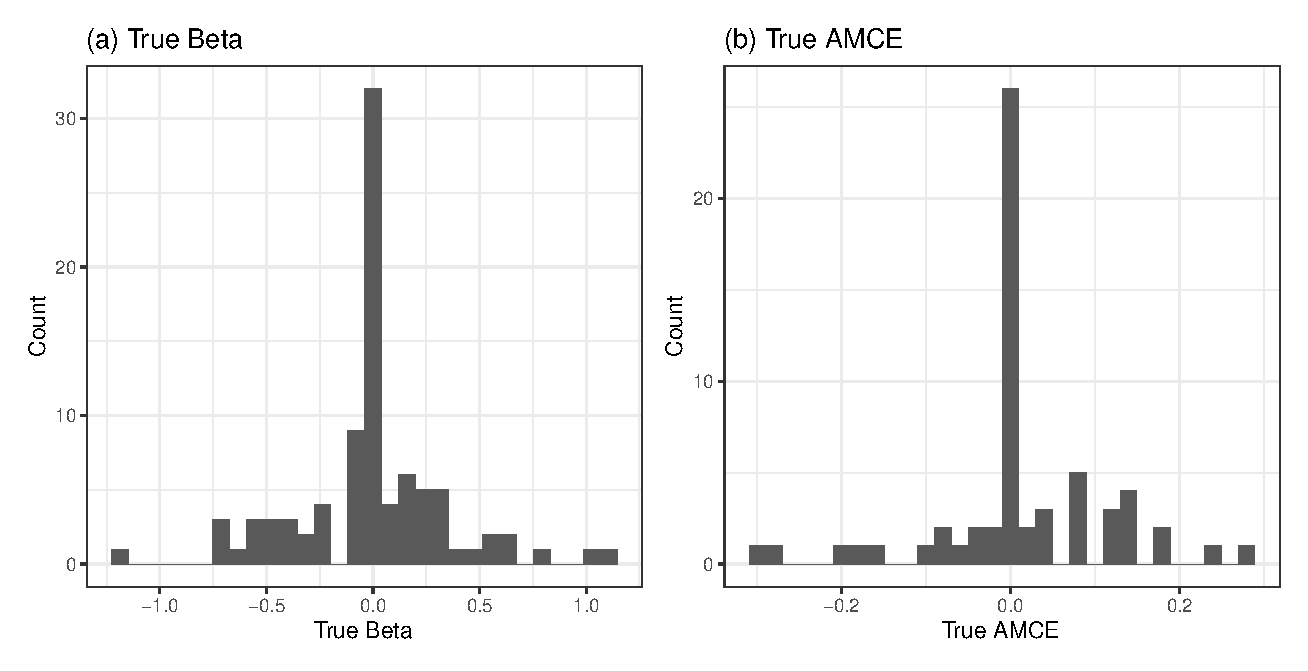
\includegraphics[width=\textwidth]{figures/sim_truth.eps}
\end{figure}

For each simulation, we draw $N'$ individuals who rate $T'$ profiles where $(N', T') \in \{(1000,5), (2000, 10)\}$. For each individual $i'$, we draw its moderators $\bm{x}_{i'}$ from a correlated multivariate normal where $\bm{x}_{i'} \sim N(\bm{0}_5, \bm{\Sigma})$ with $\bm{\Sigma}_{ij} = 0.25^{|i-j|}$ for $i,j \in \{1, \cdots, 5\}$. The distribution of cluster assignment probabilities $\pi_{ik}$ is shown below from one million Monte Carlo simulations of $[1, \bm{x}_{i'}^\top]$.

\begin{figure}[!htbp]
	\caption{Cluster Membership Probabilities}
	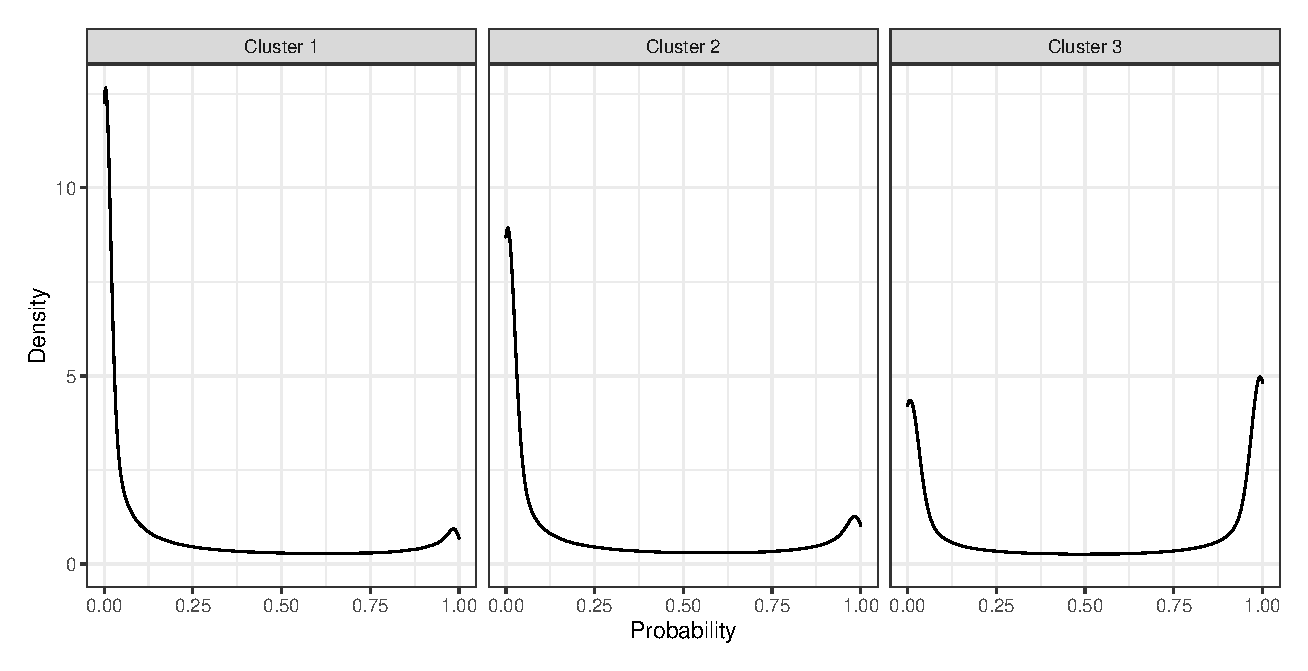
\includegraphics[width=\textwidth]{figures/sim_pi.eps}
\end{figure}

We see that the members are well-separated; the clusters are somewhat unbalanced, i.e. $\bar{\bm{\pi}} = [0.217, 0.261, 0.522]$. If we consider the maximum probability for each person $i$, i.e. $\pi^*_i = \max_{k \in \{1, 2, 3\}} \pi_{ik}$, this distribution has a median of 0.93, a 25th percentile of 0.75 and a 75th percentile of 0.99.

In terms of simulating the treatment profiles and outcome, for each individual $i'$, we draw their true cluster membership $z_i'$ using their $\bm{\pi}_{i'}$. For each task $t'$, we then draw a pair of treatments at random and then, given $z_i'$, draw the outcome $y_i'$ using the generative model outlined in the main text. 

After estimating our model with $K = 3$, we resolve the problem of label switching by permuting our estimate cluster labels to minimize the absolute error between the estimated posterior membership probabilities $\{E[z_{ik} | \bm{\theta}]\}_{k=1}^K$ and $\bm{z}_i'$ (the one-hot assignment of cluster membership).

\subsection{Additional Results}
\label{sec:app_simulations_coverage}

We provide additional simulations to complement the main text. Figure~\ref{fig:app_simulation_beta} presents the results for the simulations in the main text when considering the $\bm{\beta}_k$ (instead of the AMCE). It shows a similar story of some bias even at the larger sample size.

\begin{figure}[!ht]
	\centering \spacingset{1}
	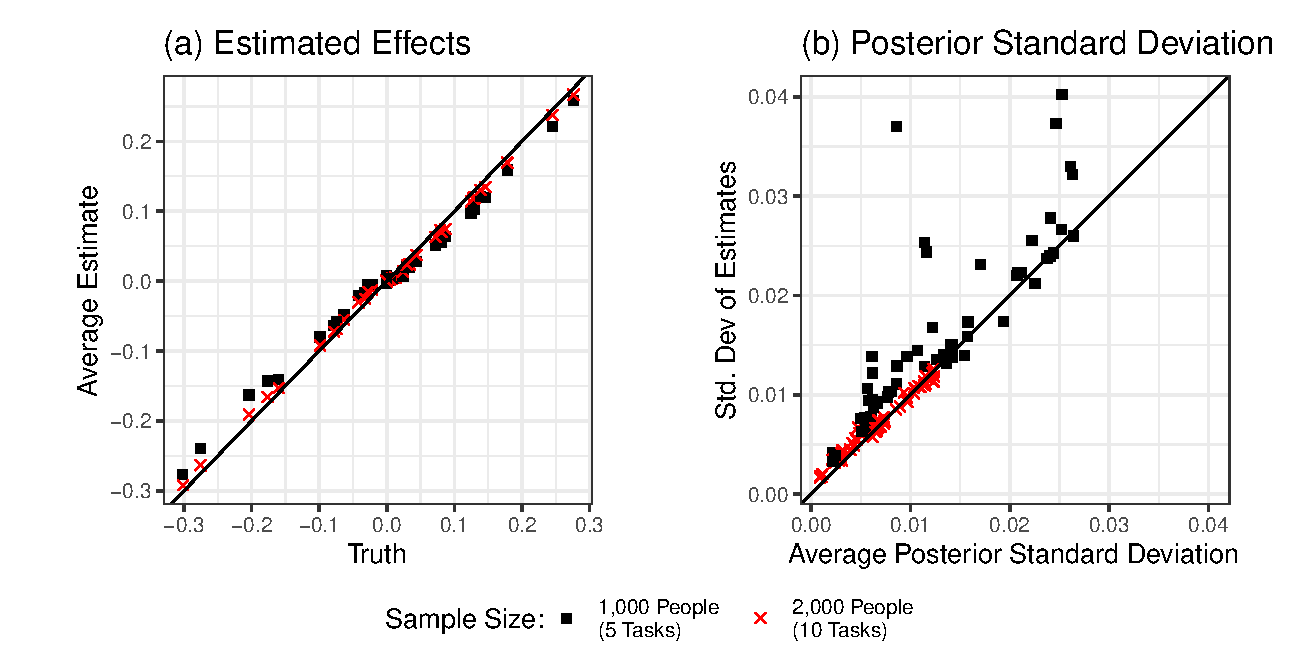
\includegraphics[width=\textwidth]{figures/sim_ame.eps}
	\caption{The empirical performance of the proposed estimator on
		simulated data. The black squares indicate the effects estimated
		with the smaller sample size (1,000 people completing 5 tasks);
		the red crosses indicate effects estimated with the larger sample
		size (2,000 people completing 10 tasks).}
	\label{fig:app_simulation_beta}
\end{figure}

To address this, we consider an alternative procedure employing sample splitting. We fit the model using half of the data (selected at random) and then refit the model. To refit the model, we hold fixed the sparsity pattern estimated in the original estimation holds (i.e., which levels are fused together) using a tolerance of $10^{-3}$. We also fix the estimated moderator relationship, i.e. $\pi_{k}(\bX_i)$, and only estimate the treatment effect coefficients after fusion. Algorithm~\ref{alg:refit} states the procedure. To calculate the average marginal effects, as noted in Appendix~\ref{append:amce_acie_der}, we use the empirical distribution of treatments to marginalize over other factors. In this split version, we also use the distribution from the full dataset.

\begin{algorithm}[!ht]\spacingset{1.25}
	\caption{Refitting Procedure}
	\label{alg:refit}
	\begin{algorithmic}
		\State{1. Randomly split the observations $i \in \{1, \cdots, N\}$ into two groups indexed by $\mathcal{I}_1$ and $\mathcal{I}_2$} 
		\State{2. Using the data $i \in \mathcal{I}_1$, estimate the parameters of the model using Algorithm~\ref{alg:main} in the main text. Define the resulting parameters from this as $\tilde{\bm{\theta}}$: $\{\tilde{\bm{\beta}}_k\}_{k=1}^K$, $\{\tilde{\bm{\phi}}_k\}_{k=2}^K,~\tilde{\mu}$}
		\State{3. Fuse levels $l$ and $l'$ of factor $j$ for cluster $k$ where the following condition holds for tolerance $\epsilon$
		
		$$\max \left\{\left|\tilde{\beta}^j_{kl} - \tilde{\beta}^j_{kl'}\right|\right\} \bigcup \left\{\bigcup_{j' \neq j} \bigcup_{m=0}^{L_{j'}-1} \left| \tilde{\beta}^{jj'}_{klm} - \tilde{\beta}^{jj'}_{kl'm}\right|\right\} \leq \epsilon$$
		
		For each combination where this is satisfied, construct matrices $\bm{R}_k$ that contain the required equality constraints, i.e. where $\bm{R}_k^T\tilde{\bm{\beta}}_k$ ensures that $\tilde{\beta}^j_{kl} = \tilde{\beta}^j_{kl'} = 0$ or $\tilde{\beta}^{jj'}_{klm} - \tilde{\beta}^{jj'}_{kl'm} = 0$. 
		
		Define $\tilde{\pi}_k(\bX_i)$ as follows:
		
		$$\tilde{\pi}_k(\bX_i) = \frac{\exp(\bX_i^\top \tilde{\bphi}_k)}{\sum_{k'=1}^K
			\exp(\bX_i^\top \tilde{\bphi}_{k'})}$$	
		}
		\State{4. Using the other half of the data $i \in \mathcal{I}_2$, estimate the refit parameters for the treatment effects, where $\bC$ contains the original sum-to-zero constraints discussed in the main text.
		\begin{equation*}
		\{\hat{\bm{\beta}}^{\mathrm{refit}}_k\}_{k=1}^K, \hat{\mu}^{\mathrm{refit}} = \argmax_{\{\bm{\beta}_k\}_{k=1}^K, ~\mu}~\sum_{i \in \mathcal{I}_2} \ln \left(\sum_{k=1}^K \tilde{\pi}_k(\bm{X}_i) \zeta_k(\bm{T}_i)\right) \quad \mathrm{s.t.} \quad \bC^T \bm{\beta}_k = \bm{0},~\bm{R}_k^T\bm{\beta}_k = \bm{0}
		\end{equation*}
		}
	\end{algorithmic}
\end{algorithm}

Figure~\ref{fig:app_dist_simulations} compares the estimators from the split sample and full data (``Full Sample'', i.e. the methods shown in the main text) approaches. It shows the distribution of the root mean-squared error (RMSE), bias, and coverage across the estimated AMCE and coefficients. We split the results by whether the true underlying effect is zero to compare differences across those cases. We also consider one even larger sample size (4,000 people with 10 tasks) to examine a scenario where the split sample method has the same amount of data as the full sample method for the second step in the estimation process.

\begin{figure}
	
	\begin{subfigure}{\textwidth}	
		\caption{Results for AMCE}
		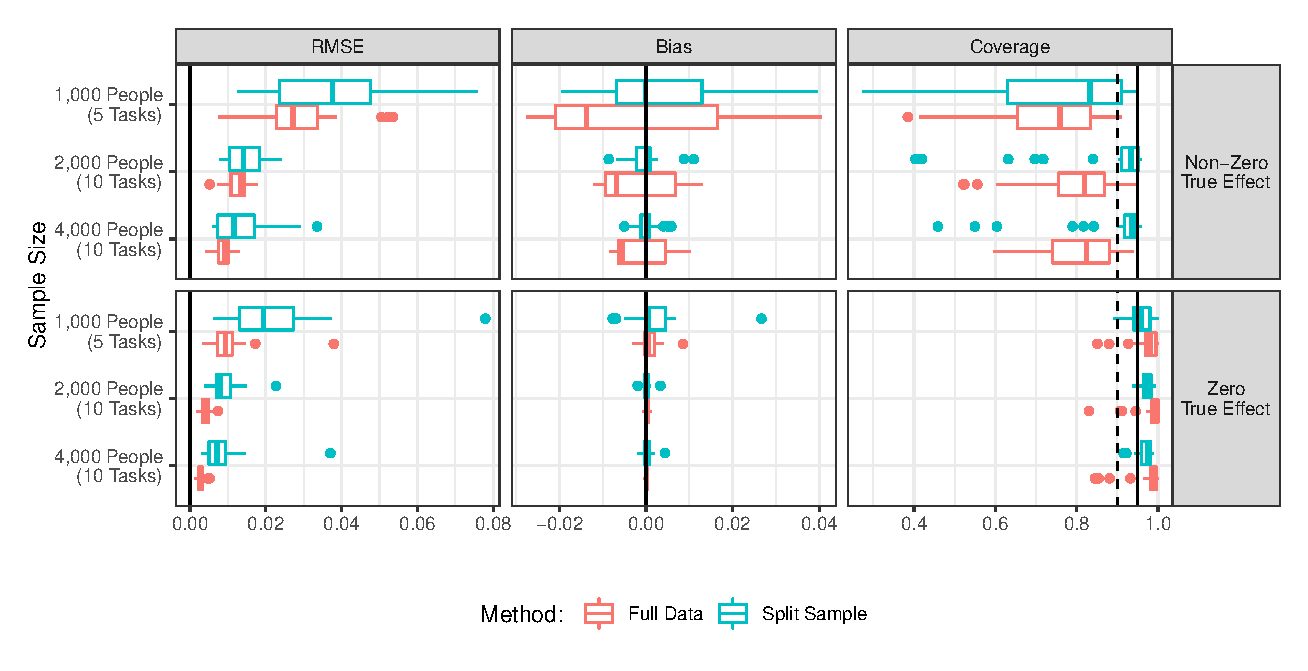
\includegraphics[width=\textwidth]{figures/app_perf_splitsample_ame.eps}
	\end{subfigure}

	\begin{subfigure}{\textwidth}	
			\caption{Results for $\bm{\beta}_k$}
			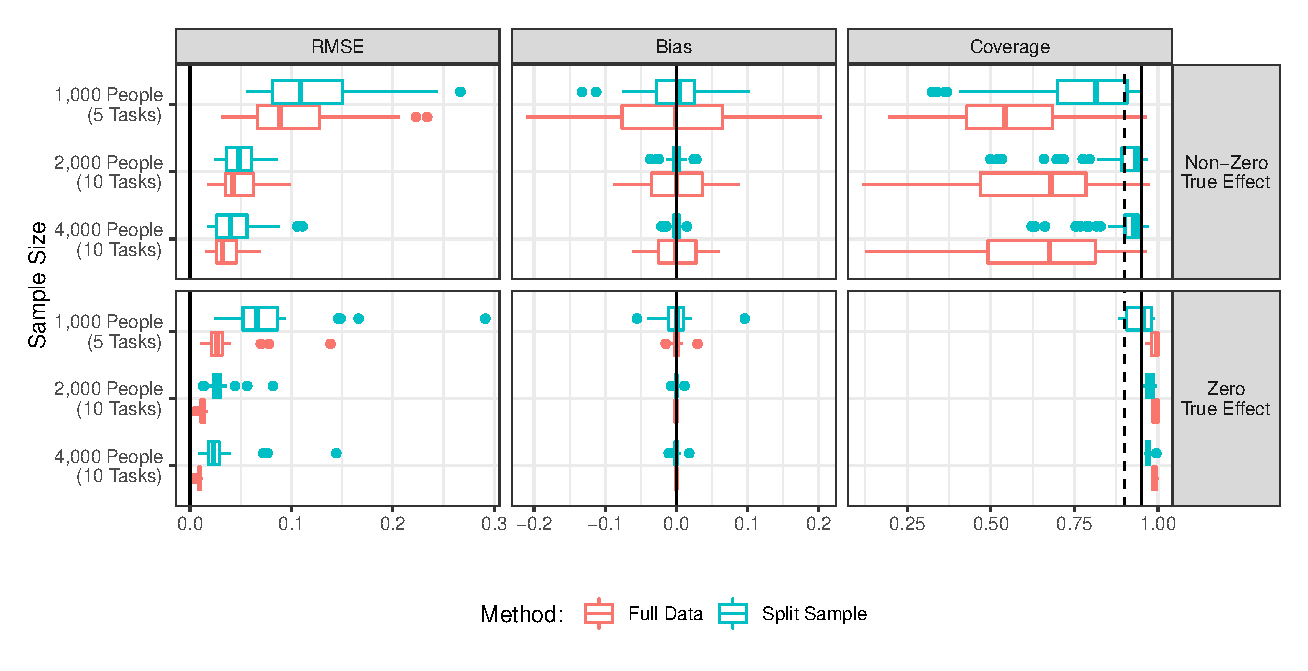
\includegraphics[width=\textwidth]{figures/app_perf_splitsample_beta.eps}
	\end{subfigure}

	\caption{The distribution of performance for each estimator across ample sizes. The top figure shows results for the AMCE; the lower figure shows results for the coefficients $\bm{\beta}_k$. Inside each figure, results are split by whether the true effect is zero (``Zero True Effect'') or not (``Non-Zero True Effect''). The boxplot shows the distribution across all effects for each cluster. For the plots on RMSE and bias, the solid vertical line indicates zero. For coverage, the solid line indicates 95\% coverage and the dashed line indicates 90\%.}\label{fig:app_dist_simulations}
\end{figure}

The figure corroborates the initial results that the full data method has non-trivial bias that decreases very slowly even at the largest sample sizes. By contrast, the bias is very small in the split sample method. As the panel on coverage shows, this results in considerably better coverage---especially for quantities with a non-zero true effect. At the two larger sample sizes, the median frequentist coverage of the split sample method is close to the nominal 95\%, with a few outliers that have low coverage. In terms of RMSE, the methods perform similarly.


\section{Additional Results for Immigration Conjoint Experiment}
\label{app:emp_marg_means}

We provide some additional results for our main empirical analysis. First, focusing on the three-cluster model, we report a different quantity of interest. We use an analogue to the ``marginal means'' estimator in \cite{leeper2020measuring}. We compute the probability of a profile being chosen \emph{without} specifying a baseline category. The equation is shown below for the forced choice case; note it consists of two of the terms used for the AMCE. 

\begin{align}
\mathrm{MM}_{jk}(l) & \ = \ \frac{1}{2}\E \left[
\left\{\Pr\left(Y_i = 1 \mid Z_i=k, T^L_{ij}=l,
\bT^L_{i,-j}, \bT^R_{i}\right) + \Pr\left(Y_i = 0 \mid Z_i=k, T^R_{ij}=l,
\bT^R_{i,-j}, \bT^L_{i}\right)
\right\}\right]. 
\end{align}

The below plot ignores randomization restrictions when estimating this quantity to center the estimate around 0.50 as in \cite{leeper2020measuring}. The results are substantively similar to the analysis in shown in the main paper using AMCEs.

\begin{figure}[t!]
	\centering \spacingset{1}
	\includegraphics[width=\textwidth]{figures/marginal_means.pdf}
	%6x8
	\caption{Estimated average marginal means using a
		three-cluster (right) analysis. The point
		estimates and 95\% Bayesian credible intervals are shown.} \label{fig:marg_means}
\end{figure}

Second, as noted in the main text, we found that sample splitting and refitting the model (see Appendix~\ref{sec:app_simulations_coverage}) was somewhat unstable given different splits of the data. To illustrate this point, Figure~\ref{fig:perm_AMCE} shows the 25th-75th percentile (and median) of the AMCEs estimated across twenty repetitions of splitting the data into halves and then using the refitting procedure described above. We address the problem of label switching using a permutation of labels that minimizes the average mean absolute error between all pairs of estimates; we find a permutation by randomly permuting the labels for a randomly chosen set of estimates and repeat this repeatedly until the average mean absolute error stabilizes. 

While Figure~\ref{fig:perm_AMCE} shows instability in some of the estimated AMCE, it broadly shows a similar result to that in the main text. For example, one cluster (Cluster 2 when $K=2$; Cluster 3 when $K=3$) shows a clear effect of country across most splits whereas one cluster (Cluster 1 when $K=2$ and Cluster 2 when $K=2$) generally shows a large penalty for immigrants who entered without legal authorization. 

\begin{figure}[!htbp]
	\centering \spacingset{1}
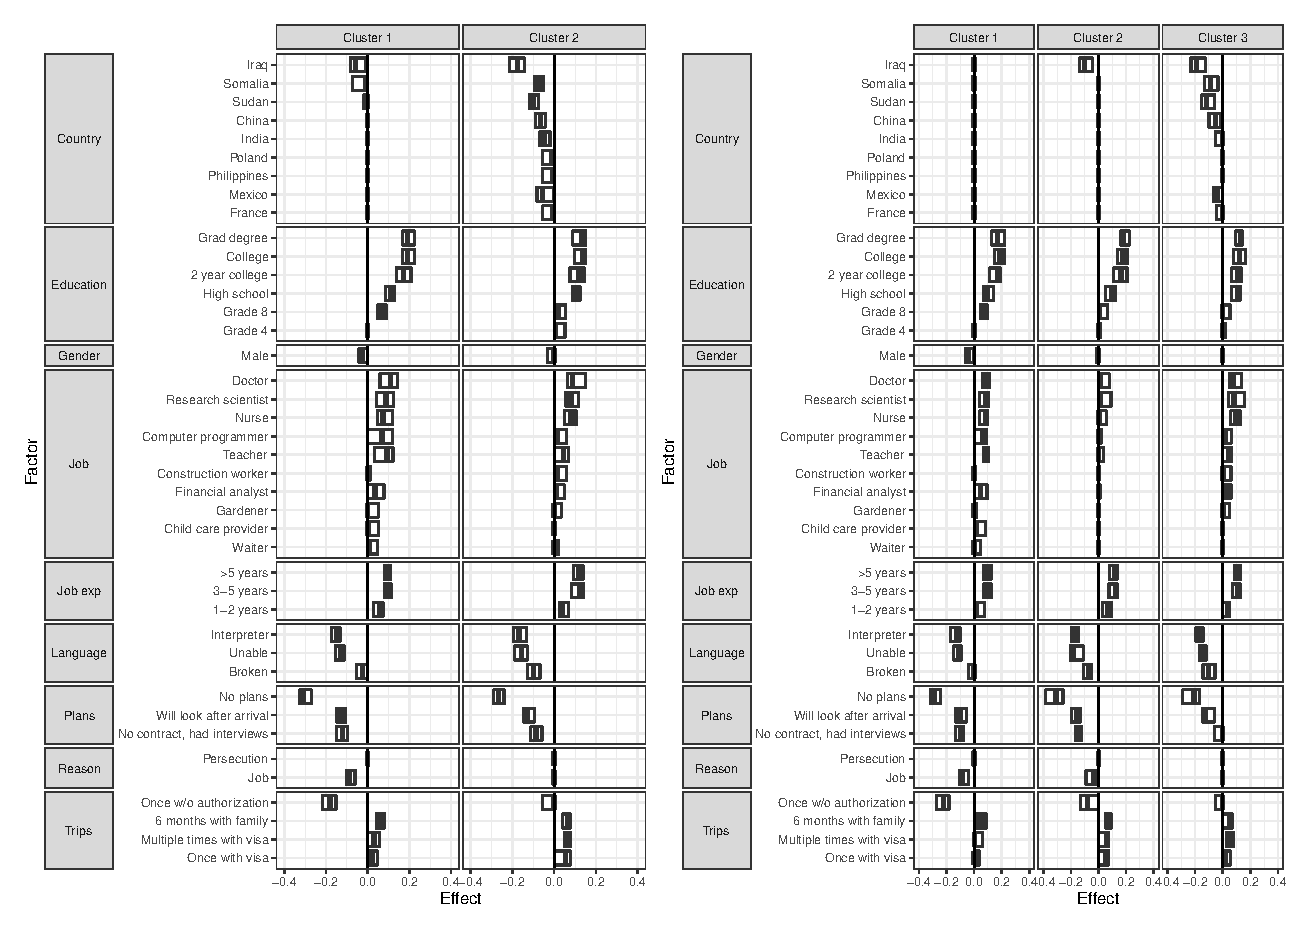
\includegraphics[width=\textwidth]{figures/app_repeat_hh_AME.eps}
%6x8
\caption{The distribution of AMCE from a two-cluster and three-cluster model with twenty random splits of the data. The interquartile range and median are shown.} \label{fig:perm_AMCE}
\end{figure}
